\section{Implementierung}

In diesem Kapitel wird die Implementierung des Projektes mit Fokussierung auf die einzelnen Komponenten beschrieben. Da eine komplett detaillierte Beschreibung des ganzen Quellcodes den Umfang dieser Ausarbeitung bei weitem sprengen würde, werden in diesem Kapitel die wichtigsten Implementierungskonzepte deren Funktionswiese, sowie deren Komponenten dargestellt. Für eine vollständig detaillierte Darstellung wird auf den Quellcode und den darin enthalten Kommentare sowie das zugehörige 
github-Wiki (https://github.com/FleeAndCatch-Dev/FleeAndCatch-Docs/wiki) verwiesen.

\subsection{Kommunikation}

Die Kommunikation der einzelnen Komponenten des Schwarmverhaltens baut auf einer klar definierten Struktur, um ein Schwarmverhalten als verteiltes System zu ermöglichen, siehe Abbildung \eqref{fig:full_classdiagram}. Die Daten werden dabei als \gls{json} Objekte zur optimalen plattformübergreifenden Interpretation versendet, wobei jeweils die entsprechende Bibliothek zur Serialisierung verwendet wird.
\begin{verbatim}
\end{verbatim}
\begin{figure}[h]
	\begin{center}
		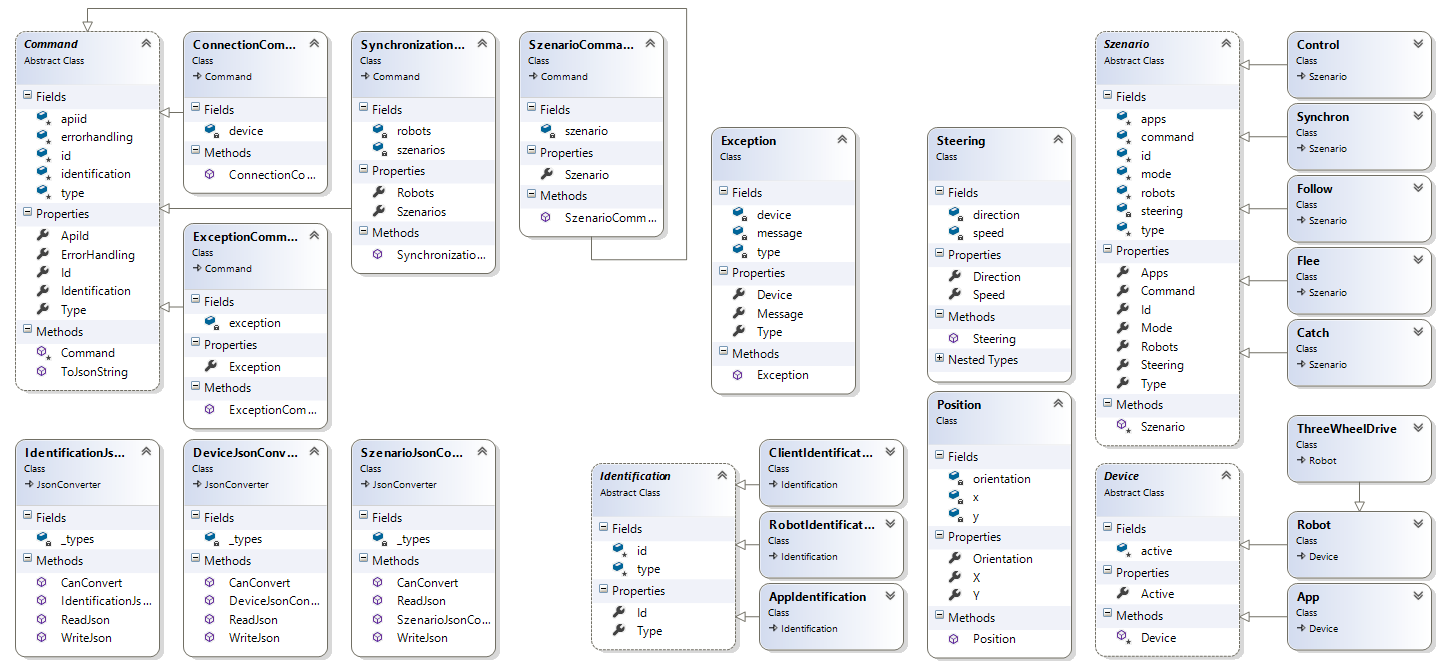
\includegraphics[width=0.95\textwidth]{images/uml/full_class_diagram.png}
	\end{center}
	\caption{Aufbau Commands}
	\label{fig:full_classdiagram}
\end{figure}

\newpage
\noindent
Der Kern zur Implementierung der Kommunikation erfolgt in zwei Methoden, die auf jeder Komponente zur Verfügung stehen. Diese dienen zum Versenden, sowie Empfangen von Daten, wobei diese als Zeichenkette serialisiert und in Bytes aufgeteilt werden, siehe Abbildung \eqref{fig:SendCommand}. Um den vollständigen Umfang der Daten zu erfassen, wird die Größe ermittelt und standardmäßig mittels vier Bytes übertragen. Dadurch ist eine maximale Paketgröße von 32 Byte möglich, was einer Länge von etwa 4 Milliarden Zeichen entspricht. Die Interpretation zum Empfangen erfolgt mit ähnlichem Muster, indem zunächst die Größe der Daten festgestellt wird und die Daten deserialiert werden, siehe Abbildung \eqref{fig:ReceiveCommand}.

\begin{figure}[h]
	\centering
	\subfloat[Versende Kommando]{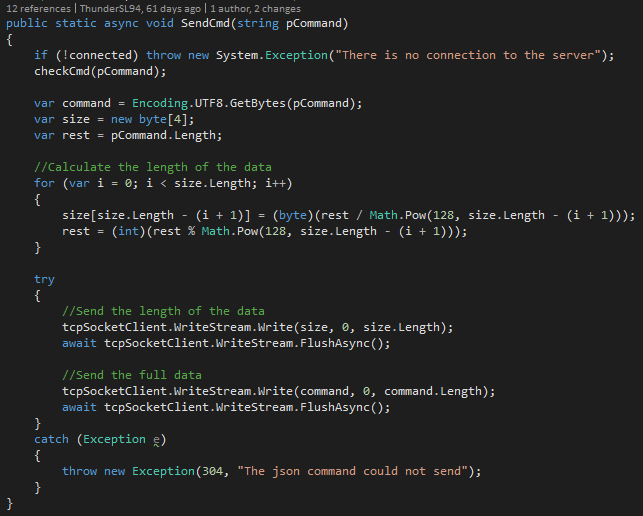
\includegraphics[width=0.6\textwidth]{images/code/SendCommand.png}\label{fig:SendCommand}}
	\qquad
	\subfloat[Empfange Kommando]{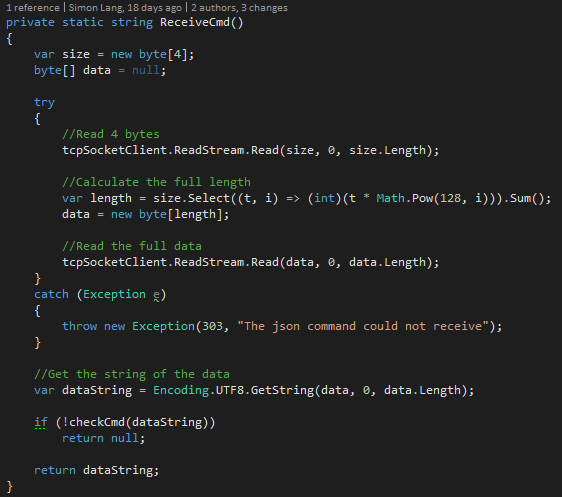
\includegraphics[width=0.6\textwidth]{images/code/ReceiveCommand.png}\label{fig:ReceiveCommand}}
	\caption{Kommunikation}
\end{figure}

\newpage
\paragraph{Kommandos}

\begin{wrapfigure}{r}{0.55\textwidth}
	\begin{center}
		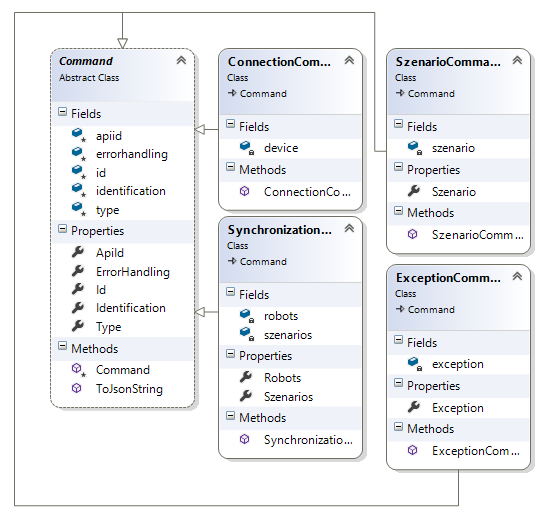
\includegraphics[width=0.5\textwidth]{images/uml/commands.png}
	\end{center}
	\caption{Kommandos}
	\label{fig:commands_classdiagram}
	\begin{center}
		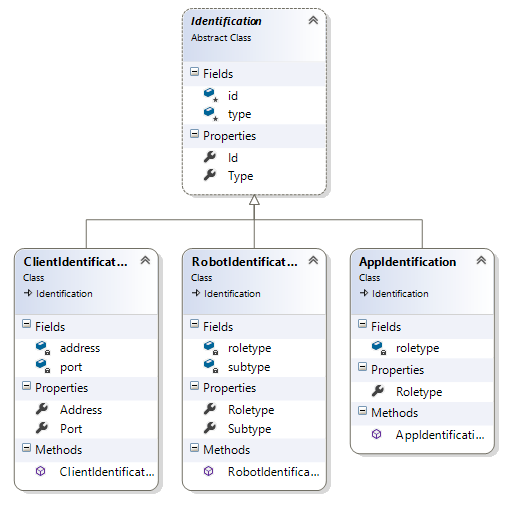
\includegraphics[width=0.5\textwidth]{images/uml/identification.png}
	\end{center}
	\caption{Identifikation}
	\label{fig:identification_classdiagram}
\end{wrapfigure}

stellen die Basis der Kommunikationsstruktur sowie den aktuellen Kontext dar, indem sich die Software befindet, siehe Abbildung \eqref{fig:commands_classdiagram}. Sie enthalten grundlegende Attribute zur allgemeinen Identifikation des Kommandos, die zur Interpretation verwendet und über definierte Enums ausgewählt werden. Je nach Kommando sind zusätzliche Objekte enthalten, die durch die jeweilige Id vordefiniert sind.\\

\paragraph{Identifikationen}

stellt die individuelle Identität der einzelnen Komponente dar, siehe Abbildung \eqref{fig:identification_classdiagram}. Diese wird durch eine fortlaufende Identifikationsnummer, Typen und je nach Ableitung weiteren Attributen erreicht. Um die jeweiligen Kommandos entsprechend zuzuordnen, sind die Identifikationsobjekte in jedem Kommando vorhanden und bilden die Basisobjekte. Die unterschiedlichen Typen sind dabei für verschiedene Kontexte der Software zuständig. Die ClientIdentification stellt einerseits die Verbindung einer allgemeinen Komponente zur Desktopanwendung dar, wogegen die Robot- bzw. AppIdentification die spezifische Identifikation der Komponente darstellt. Die Erstellung der Identifikation erfolgt jeweils wiederholt zur Anmeldung der Komponente am System. Zunächst wird ein leeres Objekt erzeugt, dass anschließend durch abfragende Kommandos an die entsprechende Komponente befüllt wird, welche hinterher eine berechnete Identifikationsnummer erhält.

\newpage
\paragraph{Geräte}

\begin{wrapfigure}{r}{0.55\textwidth}
	\begin{center}
		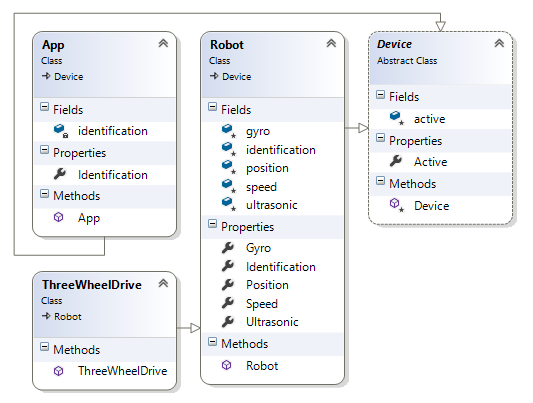
\includegraphics[width=0.5\textwidth]{images/uml/devices.png}
	\end{center}
	\caption{Devices}
	\label{fig:devices_classdiagram}
	\begin{center}
		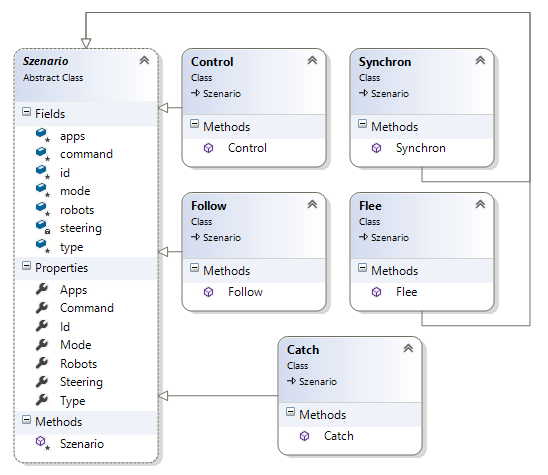
\includegraphics[width=0.5\textwidth]{images/uml/szenarios.png}
	\end{center}
	\caption{Scenarios}
	\label{fig:szenarios_classdiagram}
\end{wrapfigure}

stellen die Komponenten dar, die an einem Szenario eines Schwarmverhaltens teilnehmen, siehe Abbildung \eqref{fig:devices_classdiagram}. Sie enthalten jeweils spezifische Identifikations Objekte, zur gegenseitigen Zuordnung, sowie die erfassten Daten der entsprechenden Komponenten. Die Unterscheidung erfolgt in zwei Typen, dem Robot und der App, wobei der Roboter in seine jeweiligen Untertypen gegliedert werden kann. 

\paragraph{Szenarios}

stellen den Ablauf des Schwarmverhaltens dar, in dem sich der Nutzer befindet, siehe Abbildung \eqref{fig:szenarios_classdiagram}. Sie enthalten die jeweiligen Teilnehmer des Szenarios, sowie die Steuerungsinformationen und damit die gesamten Daten des aktuellen Kontextes. Diese Objekte werden laufend aktualisiert und besitzen lediglich zur Laufzeit des Szenarios ihre Gültigkeit. Dabei existieren verschiedene Kategorien von Szenarien, siehe Abschnitt \eqref{szenarien}. Diese definieren jeweils einen unterschiedlichen Kontext und besitzen daher je nach Szenario zusätzliche Attribute.

\newpage
\paragraph{Konverter}

\begin{wrapfigure}{r}{0.55\textwidth}
	\begin{center}
		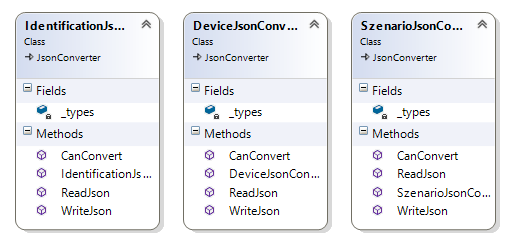
\includegraphics[width=0.5\textwidth]{images/uml/json_converter.png}
	\end{center}
	\caption{JsonConverter}
	\label{fig:converter_classdiagram}
\end{wrapfigure}

dienen der Deserialisierung von abstrakten \gls{json} Objekten, welche nicht direkt identifiziert werden können, siehe Abbildung \eqref{fig:converter_classdiagram}. Dazu gehören abstrakte Klassen, sowie Schnittstellen, welche keinem spezifischen Objekt zugeordnet werden können. Die Implementierung erfolgt durch die Überschreibung der entsprechenden Methoden zur Deserialisierung und Serialisierung, siehe Abbildung \eqref{fig:ConverterRead} und \eqref{fig:ConverterWrite}. Je nach Anwendung, wird ein Parameter übergeben, der das Objekt als Zeichenkette beinhaltet. Dieses wird durch eine Abfolge von Bedingungen auf den Typen geprüft, um das Objekt zu erstellen.\\

\begin{figure}[h]
	\centering
	\subfloat[ReadJson]{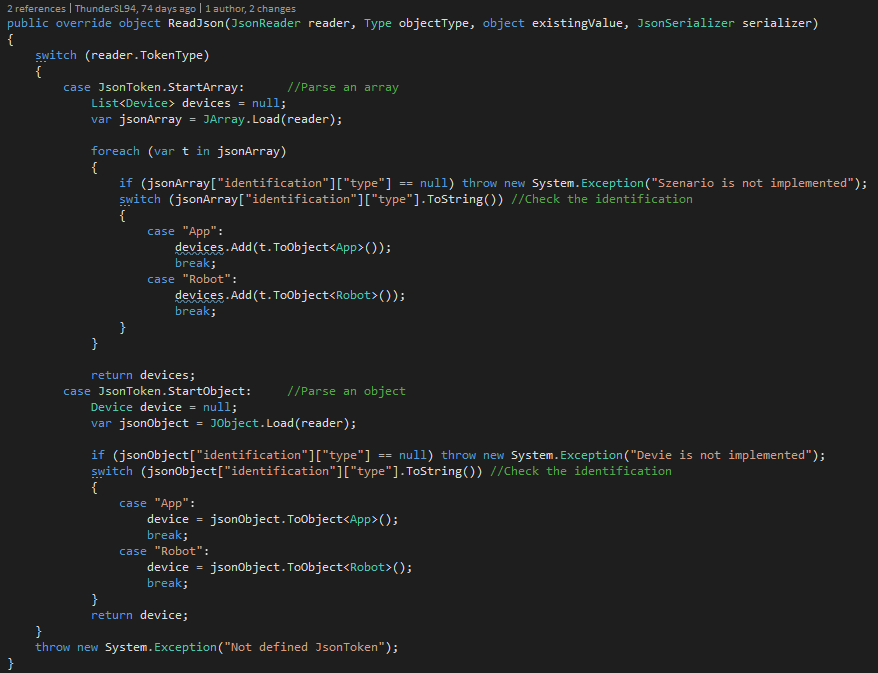
\includegraphics[width=0.7\textwidth]{images/code/DeviceConverterRead.png}\label{fig:ConverterRead}}
	\qquad
	\subfloat[WriteJson]{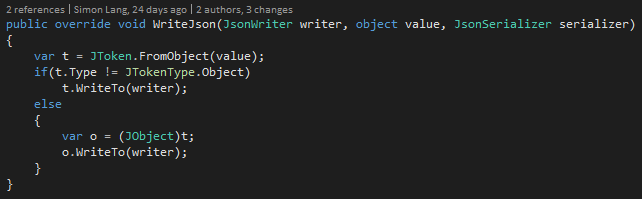
\includegraphics[width=0.7\textwidth]{images/code/DeviceConverterWrite.png}\label{fig:ConverterWrite}}
	\caption{Device JsonConverter}
\end{figure}

\newpage
\subsection{\gls{app}}

Die Erstellung der \gls{app} erfolgt in einer plattformübergreifenden Implementierung durch Xamarin in C\#. Kernelemente stellen hierbei die Struktur, Oberfläche, Businesslogik sowie das Kommunikationssystem dar. Durch die zentrale Verwendung des Kommunikationssystems wird dieses in ein separates Projekt untergliedert, siehe Abbildung \eqref{fig:solution} und wird als solches von der \gls{app} als Bibliothek eingebunden. Somit lässt sich die Logik einmalig implementieren und kann auf andere Systemen entsprechend übertragen werden.\\
Die \gls{app} setzt sich aus vier verschiedenen Projekten zusammen, einer \acrshort{pcl} als Projekt zur plattformübergreifenden Entwicklung und den plattformspezifischen Projekten. Diese werden dem Zielsystem entsprechend ausgewählt und erzeugen durch ihre bestehende Referenz auf die \acrshort{pcl} einen plattformspezifischen Quellcode als \gls{il}, der anschließend auf einer Plattform ausgeführt werden kann.

\begin{figure}[h]
	\begin{center}
		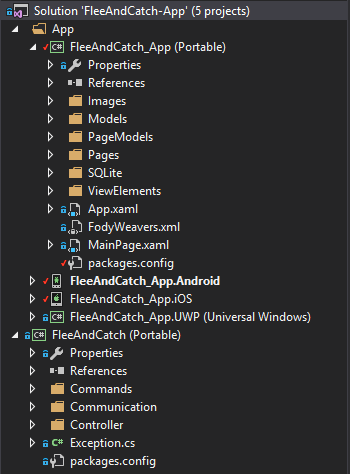
\includegraphics[width=0.5\textwidth]{images/implementation/solution.png}
	\end{center}
	\caption{Projektstruktur}
	\label{fig:solution}
\end{figure}

\newpage
\subsubsection{Workflow} %Struktur

Die Struktur der \gls{app} basiert auf dem in Xamarin verbreiteten Design Pattern \acrlong{mvvm}, welches durch ein Benachrichtigungssystem zwischen den verschiedenen Strukturen der \gls{app} eine Abspaltung der Daten, \gls{gui} und dem Businesscode erlaubt. Zusätzlich wird die standardmäßig vorhandene CodeBehind Struktur der einzelnen Seiten verwendet, wobei der Businesscode an das Layout der Seite gebunden ist, damit diese miteinander interagieren können. Zur lokalen Speicherung der Daten wird SQLite durch eine implementierte Schnittstelle verwendet, welche plattformübergreifend ansprechbar ist.

\paragraph{\acrfull{mvvm}}

stellt ein Design Pattern dar, welches eine grundlegende Struktur im Quellcode ermöglicht, siehe Abbildung \eqref{fig:mvvm}. Dabei wird die erstellte Benutzeroberfläche von der Logik, sowie den Daten getrennt, um Änderungen unabhängig voneinander durchführen zu können. Die einzelnen Objekte werden dabei durch Referenzen verbunden um diese durch Events entsprechend zu aktualisieren.\\

\begin{tabular}{p{2.5cm} p{12.25cm}}
	\textbf{Model:} & Datenschicht, welche durch den Benutzer über die \gls{gui} verändert werden kann und über Datenänderungen die entsprechenden Elemente benachrichtigt \\
	\textbf{View:} & \gls{gui} mit den anzuzeigenden Elementen, welche an das ViewModel gebunden sind und der Benutzerinteraktion dienen. \\
	\textbf{ViewModel:} & Logik des \gls{ui} als zentrale Schnittstelle zwischen dem Model und der View zum Austausch von Informationen, indem entsprechende Methoden und Dienste ausgeführt werden. \\
\end{tabular}

\bigskip

\begin{figure}[h]
	\begin{center}
		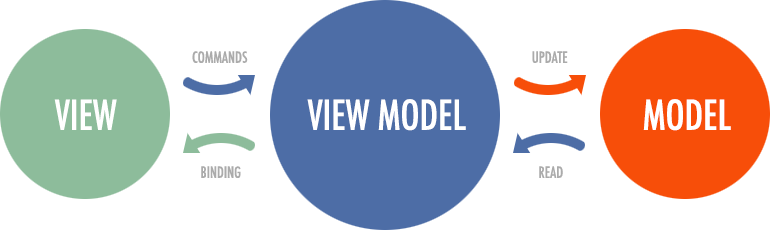
\includegraphics[width=0.95\textwidth]{images/implementation/mvvm.png}
	\end{center}	
	\caption{\acrlong{mvvm} \cite{Brecht.MVVMEntity}}
	\label{fig:mvvm}
\end{figure}

\newpage
\subsubsection{\acrfull{gui}} %Oberfläche

Die Oberfläche der \gls{app} wird mittels \gls{xaml} durch verschiedene von Xamarin zur Verfügung gestellten Elementen realisiert. Da eine \gls{app} ein einfaches Bedienkonzept voraussetzt, damit es von jedem beliebigen Benutzer verwendet werden kann, wird in diesem Projekt, auf das Navigationsprinzip der NavigationPage gesetzt. Die Navigation wird dabei durch das Aufbauen eines Stapels realisiert, was durch das Prinzip eines Stacks in der Programmierung weit verbreitet ist. Dabei wird durch den Aufruf eines Push auf eine neue Seite gewechselt, wobei der Vorgänger deaktiviert und hinter die neue im Speicher angeordnet wird, siehe Abbildung \eqref{fig:push}. Dies wird Programm technisch durch eine Liste realisiert, welche langsam aufgebaut wird. Um nun auf den Vorgänger zurück zu gelangen, wird ein Pop verwendet, um die aktuelle Seite sowie deren Daten zu löschen, wobei die vorherige Seite aus dem Speicher geladen wird, siehe Abbildung \eqref{fig:pop}.\\

\begin{figure}[h]
	\begin{center}
		
\includegraphics[width=0.75\textwidth]{images/implementation/push.png}
	\end{center}	
	\caption{Wechsel auf neue Seite \cite{Xamarin.HierarchicalNavigation}}
	\label{fig:push}
	\begin{center}
		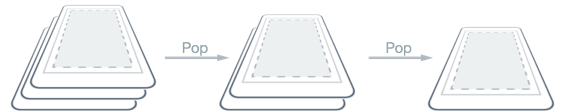
\includegraphics[width=0.75\textwidth]{images/implementation/pop.png}
	\end{center}	
	\caption{Wechsel auf alte Seite \cite{Xamarin.HierarchicalNavigation}}
	\label{fig:pop}
\end{figure}

\bigskip

\begin{wrapfigure}{r}{0.5\textwidth}
	\begin{center}
		\vspace{-1cm}
		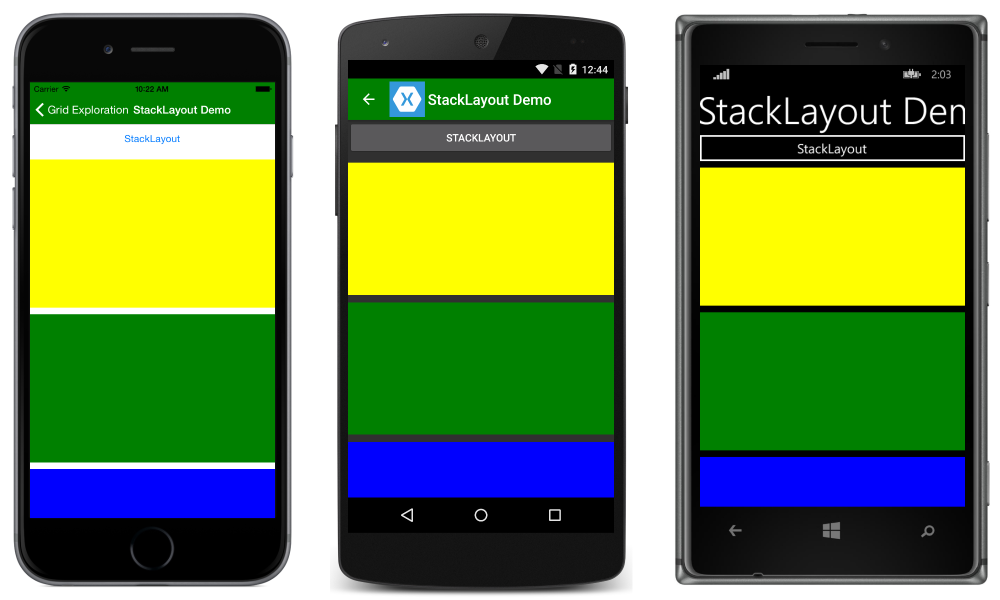
\includegraphics[width=0.45\textwidth]{images/implementation/stacklayout.png}
	\end{center}
	\caption{StackLayout \cite{Xamarin.StackLayoutXamarin}}
	\label{fig:stacklayout}
\end{wrapfigure}

\noindent
Für das Layout der einzelnen Seiten wird vor allem auf das StackLayout gesetzt. Dieses ist einfach umzusetzen, indem eine vertikale oder horizontale Orientierung zur Anordnung der verschiedenen Elemente festgelegt wird, welche entsprechend ihrer Folge hinzugefügt werden. Zusätzlich können standardmäßige Positionierungen verwendet werden, um das Layout individuell zu beeinflussen.

\begin{verbatim}
\end{verbatim}
\newpage
\paragraph{Die SignIn Page} stellt die Benutzerschnittstelle zur Anmeldung des Nutzers am System dar, siehe Abbildung \eqref{fig:signin}. Dabei gibt dieser die entsprechende \gls{ip}-Adresse der laufenden Desktopanwendung zur Verbindung an. Durch eine implementierte Logik wird diese \gls{ip}-Adresse auf ihre Richtigkeit geprüft und die Verbindung gestartet. Bei einer erfolgreichen Verbindung wird der Benutzer zur Hauptseite weitergeleitet, wodurch ihm die entsprechenden Funktionalitäten zur Verfügung stehen. Andernfalls erscheint nach einem definierten Timeout von drei Sekunden eine Fehlermeldung, welche dem User Informationen zum Fehler vorlegt. Durch ein Switch Element ist zusätzlich die Speicherung der \gls{ip}-Adresse in einer lokalen Datenbank gegeben, wobei diese bei Start der \gls{app} automatisch geladen und eingefügt wird.\\

\begin{figure}[h]
	\begin{center}
		
\includegraphics[width=0.4\textwidth]{images/implementation/signin.png}
	\end{center}	
	\caption{SignIn Page}
	\label{fig:signin}
\end{figure}

\newpage
\paragraph{Die Home Page} stellt die Hauptseite mit der grundlegenden Navigation der \gls{app} dar, siehe Abbildung \eqref{fig:home}. Dabei hat der Benutzer die Möglichkeit ein neues Szenario eines Schwarmverhaltens zu starten, Informationen über die \gls{app} abzurufen, oder sich vom aktuelles System abzumelden.

\paragraph{Die Option Page} stellt die Benutzerschnittstelle dar, welche diesen durch die vorhandenen Szenarien anhand eines Carousels leitet, siehe Abbildung \eqref{fig:option}. Der Nutzer kann damit ein beliebiges Szenario auswählen und die Konfiguration des Schwarmes beginnen.\\

\bigskip

\begin{figure}[h]
	\centering
	\subfloat[Home Page]{
\includegraphics[width=0.4\textwidth]{images/implementation/home.png}\label{fig:home}}
	\qquad
	\subfloat[Option Page]{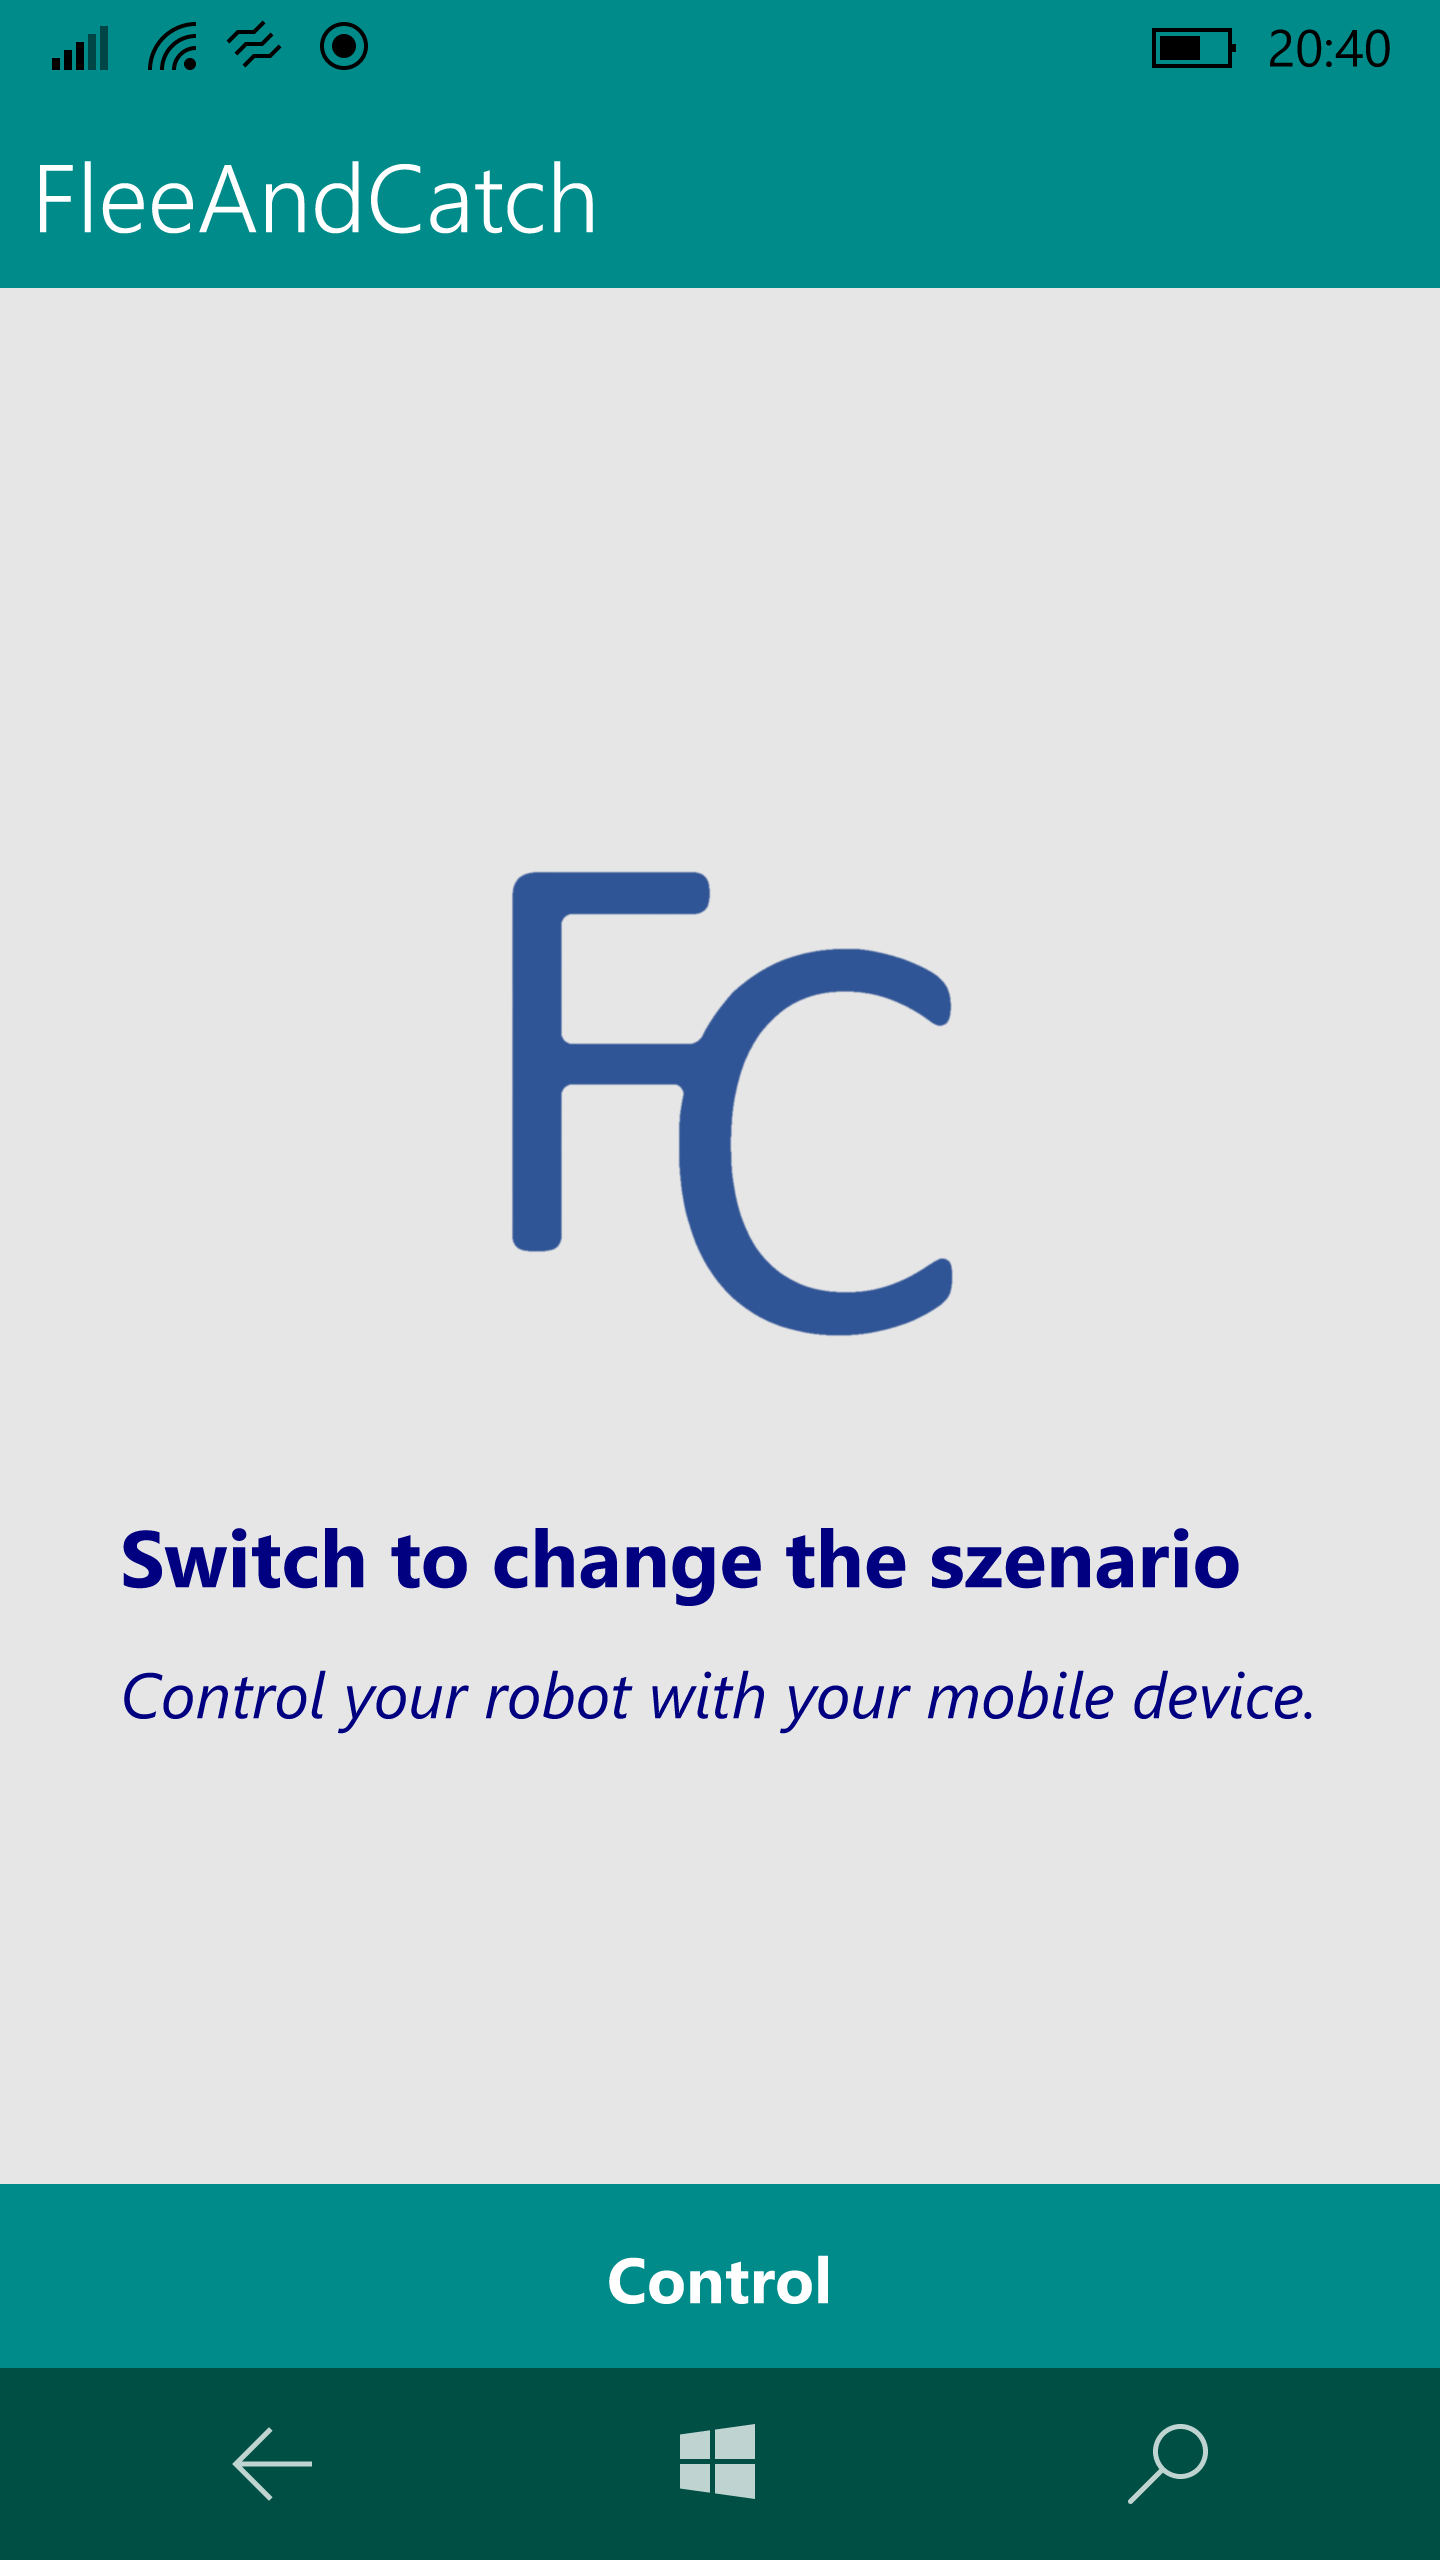
\includegraphics[width=0.4\textwidth]{images/implementation/option.png}\label{fig:option}}
	\caption{Hauptseiten}
\end{figure}

\newpage
\paragraph{Die List Page} stellt die Benutzerschnittstelle zur Auswahl der Roboter dar, welche im Szenario involviert sein sollen. Dabei kann der Benutzer unter den verschiedenen Typen wählen, wobei die Anzahl der Roboter vom gewählten Szenario abhängt. Sollte eine ungültige Anzahl an Robotern eingegeben werden, erhält der Benutzer eine Rückmeldung über eine Fehlermeldung und kann dies korrigieren. Bei korrekter Eingabe wird der Benutzer auf eine Seite mit sämtlichen Informationen des Szenarios weitergeleitet und kann dieses starten.\\

\bigskip

\begin{figure}[h]
	\begin{center}
		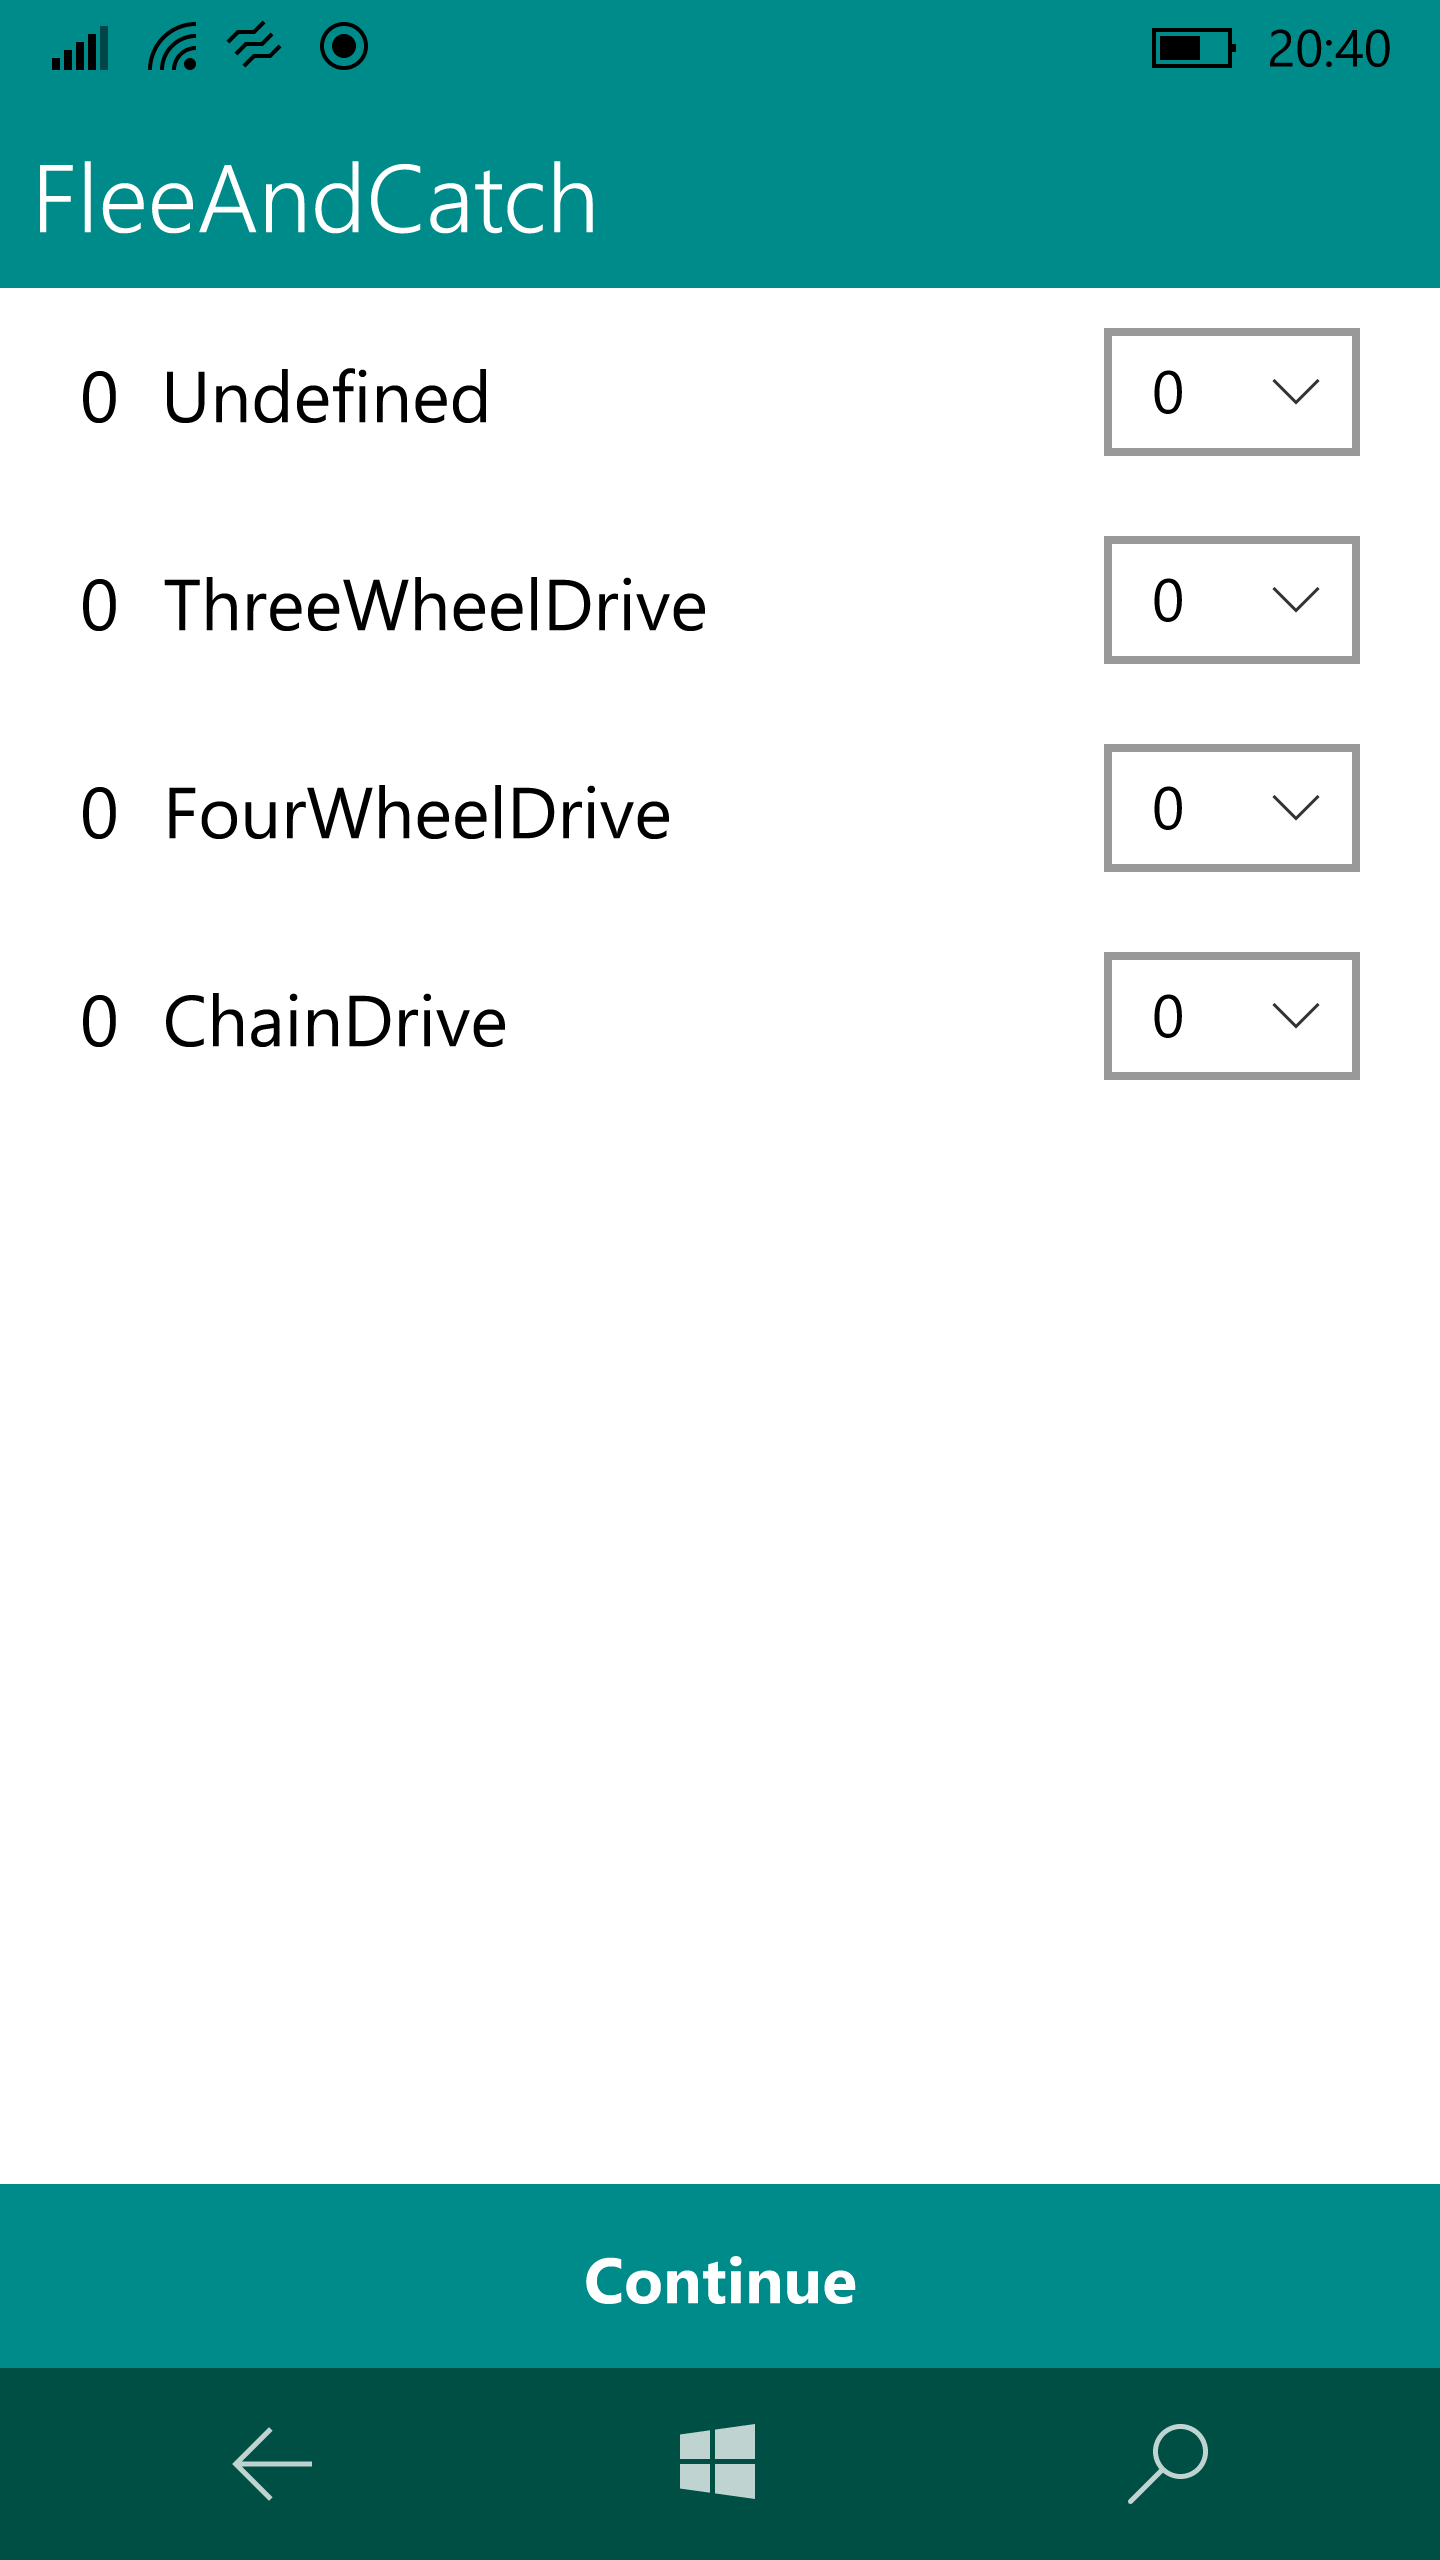
\includegraphics[width=0.4\textwidth]{images/implementation/list.png}
	\end{center}	
	\caption{List Page}
	\label{fig:list}
\end{figure}

\newpage
\paragraph{Die Szenario Page} stellt die Benutzerschnittstelle dar, welche einerseits zur Steuerung und der Überwachung des Schwarmverhaltens dient. Dabei werden laufend die Daten der Roboter, die auf dem \gls{gui} zu sehen sind aktualisiert und entsprechend angezeigt. Die Neigungssensoren des Gerätes, auf dessen Gerät die \gls{app} ausgeführt wird, ermöglichen die Roboter zu steuern, wobei die Richtung und Beschleunigung durch einen Pfeil auf der Oberfläche dargestellt werden. Der Schwarm verhält sich dabei dem entsprechenden Kontext, welchen der Benutzer zuvor eingestellt hat.\\

\bigskip

\begin{figure}[h]
	\begin{center}
		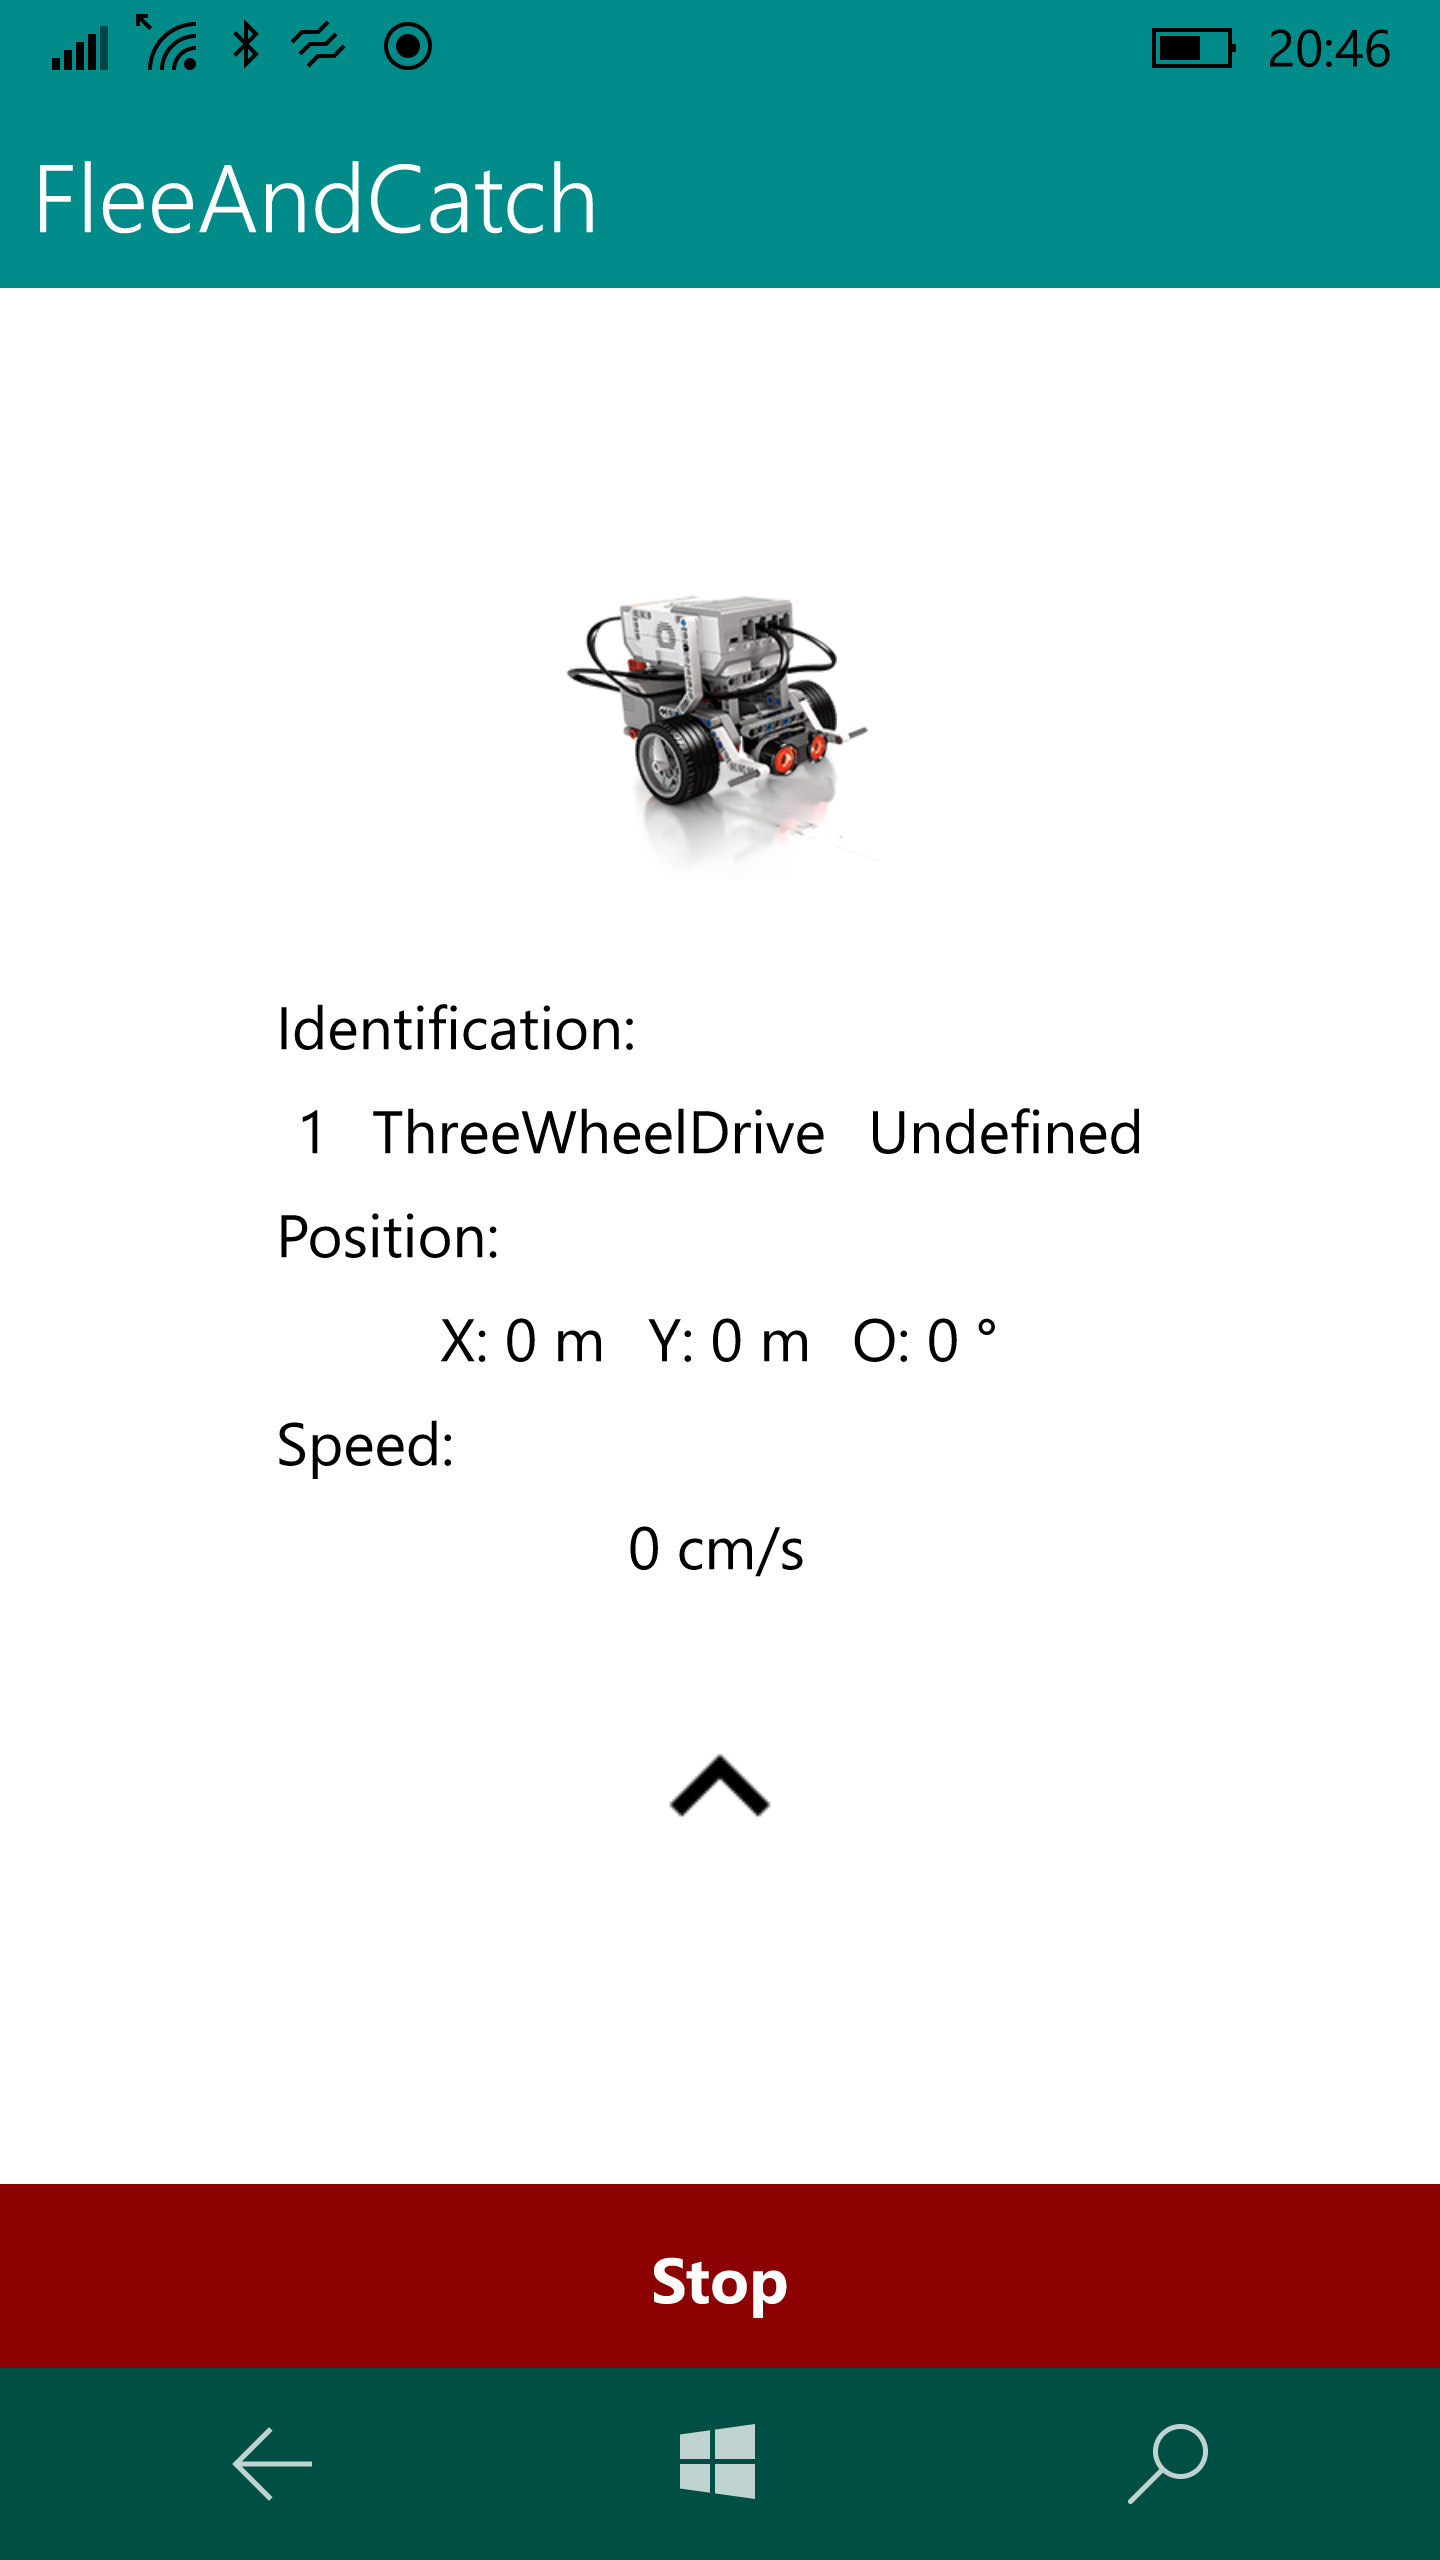
\includegraphics[width=0.4\textwidth]{images/implementation/szenario.png}
	\end{center}	
	\caption{Szenario Page}
	\label{fig:szenario}
\end{figure}

\newpage
\subsubsection{Buisnesslogic} %Logik

Die Logik der \gls{app} wird mittels des .NET \gls{framework} in C\# implementiert und ist durch die Strukturierung des \gls{mvvm} Design Pattern in separate Klassen sowie anhand eines Projektes untergliedert, welches als Bibliothek eingebunden wird. Diese Logik kann in drei Benutzerszenarien gruppiert werden.
\begin{enumerate}
	\item Anmeldung am System
	\item Erstellung eines Szenario
	\item Ablauf eines Szenario
\end{enumerate}

\begin{wrapfigure}{r}{0.5\textwidth}
	\begin{center}
		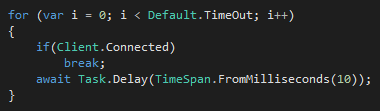
\includegraphics[width=0.45\textwidth]{images/implementation/timeout_app.png}
	\end{center}
	\caption{Timeout der Verbindung}
	\label{fig:timeout_app}
\end{wrapfigure}

\paragraph{Die Anmeldung am System} beginnt mit der Validierung der vom Nutzer eingegebenen \gls{ip}-Adresse. Identifiziert wird diese durch die Unterteilung der Zeichenkette in vier Bereiche, welche als Zahl erkannt, und durch einen Punkt abgetrennt sind sowie einen Wertebereich von 0 bis 255 besitzen. Anschließend wird die Verbindung entsprechend konfiguriert, siehe Abbildung \eqref{fig:connect_app} und durch den Aufruf der Methode ConnectAsync() gestartet. Dabei wartet die \gls{app} eine im System fest definierte Zeit von drei Sekunden, siehe Abbildung \eqref{fig:timeout_app}, bis ein Timeout als Fehler geworfen wird, um einen neuen Verbindungsversuch starten zu können.

\begin{figure}[h]
	\begin{center}
		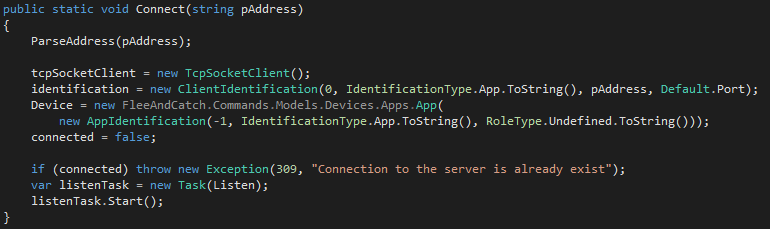
\includegraphics[width=0.9\textwidth]{images/implementation/connect_app.png}
	\end{center}	
	\caption{Verbindungsaufbau}
	\label{fig:connect_app}
\end{figure}

\noindent
Durch die Speicherung der Verbindung in einer lokalen Datenbank mittels SQLite, siehe Abbildung \eqref{fig:saveip} und \eqref{fig:sqlite} besteht die Möglichkeit eine einmal eingegebene \gls{ip}-Adresse beim Start der \gls{app} wieder zu laden, um diese nicht laufend eingeben zu müssen. Dafür wird eine entsprechende Klasse implementiert, welche die benötigten Daten als Objekt darstellt. Diese Daten werden als Tabellen in der Datenbank ablegt sowie Methoden zu deren Verwaltung bereitgestellt.

\begin{figure}[h]
	\begin{center}
		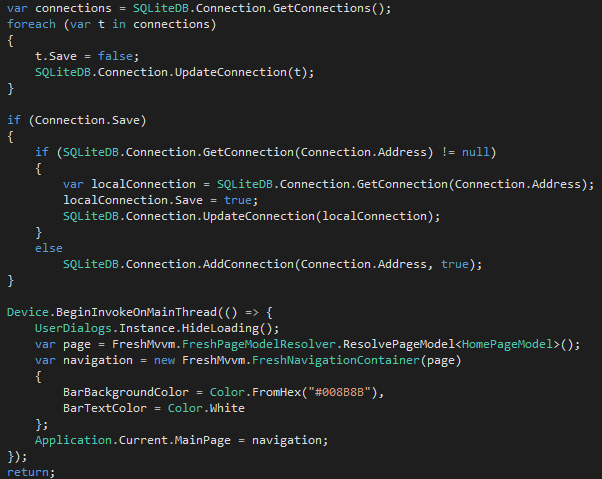
\includegraphics[width=0.8\textwidth]{images/implementation/authorization.png}
	\end{center}	
	\caption{Speicherung der \gls{ip}-Adresse}
	\label{fig:saveip}
	\begin{center}
		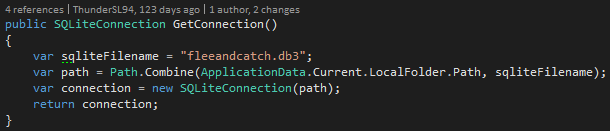
\includegraphics[width=0.8\textwidth]{images/implementation/sqlite.png}
	\end{center}	
	\caption{Definition von SQLite}
	\label{fig:sqlite}
\end{figure}

\noindent
Sobald eine \gls{app} sich erfolgreich mit dem System verbunden hat, läuft neben dem eigentlichen Hauptprozess, welchen der Nutzer durch seine Eingaben steuert ein Nebenprozess. Dieser wartet auf eingehende Kommandos und interpretiert diese nach einem festgelegten Bedingungen in der Interpreter Klasse, um entsprechend zu reagieren oder den Nutzer zu informieren sowie neue Daten anzuzeigen.

\paragraph{Die Erstellung eines Szenario} beginnt mit der Auswahl eines definierten Typ, wobei jeder einen anderen Kontext besitzt, siehe Abschnitt \eqref{szenarien}. Anschließend gelangt der Nutzer zur Auswahl der verschiedenen Roboter, welche im Szenario teilnehmen sollen. Hierbei wird die entsprechende Zahl an Robotern eines Typs einer Liste hinzugefügt, welche der Nutzer durch die \gls{gui} auswählt, siehe Abbildung \eqref{fig:addrobots}. Sollte der Nutzer dabei eine ungültige Anzahl auswählen, erhält er eine entsprechende Rückmeldung, um eine Korrektur vorzunehmen. Bei erfolgreicher Überprüfung wird das Szenario als Objekt erstellt und enthält somit alle Komponenten sowie zusätzliche Informationen zur Identifikation.

\begin{figure}[h]
	\begin{center}
		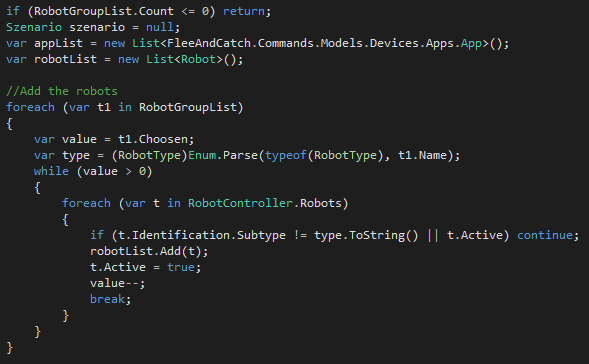
\includegraphics[width=0.8\textwidth]{images/implementation/robotlist_add.png}
	\end{center}	
	\caption{Hinzufügen der Roboter}
	\label{fig:addrobots}
\end{figure}

\noindent
Um das erzeugte Szenario zu verifizieren, wird das erzeugt Objekt an die Desktopanwendung versendet, siehe Abbildung \eqref{fig:tryszenario}, welche sämtliche beinhalteten Komponenten der Verfügbarkeit überprüft. Bei erfolgreicher Überprüfung wird der Nutzer zum Start des Szenarios mit einem Überblick auf sämtliche Informationen weitergeleitet. Andernfalls wird die Erstellung abgebrochen und der Nutzer kann Änderungen durchführen.

\begin{figure}[h]
	\begin{center}
		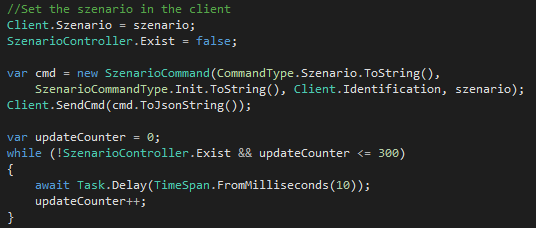
\includegraphics[width=0.7\textwidth]{images/implementation/trycreateszenario.png}
	\end{center}	
	\caption{Erstellung des Szenario}
	\label{fig:tryszenario}
\end{figure}

\paragraph{Der Ablauf eines Szenario} teilt sich in verschiedene Prozesse, wobei der Nutzer durch seine Handlungen im \gls{gui} der Hauptprozess beeinflusst. Daneben existiert ein Prozess zum Datenempfang, welcher Aktualisierungen der Daten des Schwarmes empfängt und entsprechend in der \gls{gui} einpflegt. Zur Steuerung des Schwarmes, dient ein Prozess, der mittels eines Timer laufend neu gestartet wird und somit immer neue Steuerungskommandos versendet sowie die Oberfläche der \gls{app} aktualisiert.

\begin{figure}[h]
	\begin{center}
		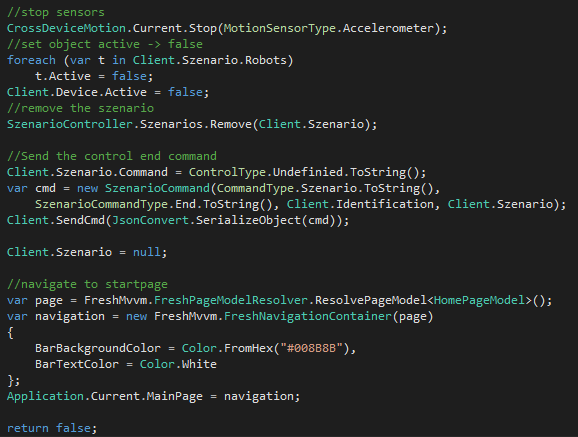
\includegraphics[width=0.7\textwidth]{images/implementation/cancelszenario.png}
	\end{center}	
	\caption{Abbruch eines Szenario}
	\label{fig:cancelszenario}
\end{figure}

\noindent
Sobald ein Szenario abgebrochen wird, müssen sämtliche Prozesse und Daten freigegeben werden, damit der Nutzer anschließend ein neues Szenario starten kann, siehe Abbildung \eqref{fig:motionvector}. Dafür wird zunächst der Neigungssensor abgeschaltet, da dieser aktuell nicht mehr benötigt wird. Zur Freigabe der Daten werden sämtliche Aktivität der Roboter abgeschaltet sowie das Szenario entfernt. Dem Backend wird anschließend das Beenden des Szenarios mitgeteilt, damit auch dieses die anderen Komponenten informieren sowie seinen reservierten Speicher freigeben kann.

\begin{figure}[h]
	\begin{center}
		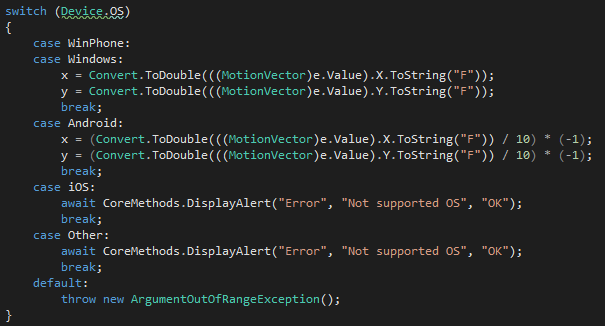
\includegraphics[width=0.7\textwidth]{images/implementation/motionvector.png}
	\end{center}	
	\caption{Neigungssensor}
	\label{fig:motionvector}
\end{figure}

\noindent
Zur Erzeugung eines neuen Steuerungskommandos, siehe Abbildung \eqref{fig:newcommand}, werden die Neigungssensoren des mobilen Gerätes verwendet. Da bei der Implementierung der Schnittstelle auf den verschiedenen Plattformen gewisse Unterschiede bestehen, müssen diese in der plattformübergreifenden Programmierung behoben werden. Dies wird durch eine Angleichung der Faktoren sowie ein Vertauschen der Attribute realisiert, wie am Beispiel von Android und Windows. Das Steuerungskommando enthält dabei keine direkten Werte, wie Geschwindigkeit und Winkel, sondern wird durch Zeichenketten (Enums) umgesetzt. Diese verändern ihre Wertigkeit entsprechend der Werten zum Neigungssensor des mobilen Gerätes.

\begin{figure}[h]
	\begin{center}
		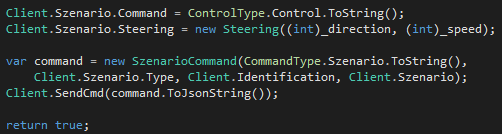
\includegraphics[width=0.7\textwidth]{images/implementation/newcommand.png}
	\end{center}	
	\caption{Neues Kommando}
	\label{fig:newcommand}
\end{figure}

\newpage
\subsection{Backend}
Das Backend ist die Kommunikations- und Verwaltungszentrale des Projekts und bildet das Rückgrat der Kommunikation. Es verwaltet die 
Devices im Kontext der einzelnen Szenarien und sorgt für den Datenaustausch zwischen den verschieden Geräten. \\
Realisiert ist des Backend wie auch der Roboter in der Programmiersprache Java. Das bringt neben der plattformunabhängigen 
Lauffähigkeit des Programms noch weitere Vorteile mit sich. So können vor allem Programmkomponenten welche die Kommunikation und
den Datenaustausch betreffen für die Implementierung des Roboterprogramms wiederverwendet werden und müssen nicht komplett neu
implementiert werden.
\subsubsection{Aufbau \& Klassenstruktur}
Die Hauptaufgabe des Backends besteht zum einen in er Verwaltung der verschiedenen Devices und zum anderen aus der Vermittlung
bzw. Verteilung der von den Geräten gesendeten Kommunikationsdaten.
\\
Aus diesem Grund wurden die Komponenten des Backendes hinsichtlich ihrer Unterstützung bei der Realisierung dieser beiden Hauptaufgaben
strukturiert und befinden sich in den folgenden Paketkategorien:
\begin{enumerate}
	%   ###############################################################################################################################
	\item{Kommunikation (\code{flee\_and\_catch.backend.communication})}
	%   ###############################################################################################################################
	\item{Verwaltung von Devices \& Szenarien (\code{flee\_and\_catch.backend.controller})}
	%   ###############################################################################################################################
\end{enumerate}
Davon unabhängig existieren noch Komponenten die zur Realisierung einer grafische Benutzeroberfläche dienen und sich im Paket 
\code{backend.view} befinden, diese ist jedoch 
unabhängig von der eigentlichen Programmlogik des Backendes und dient vorrangig dem Monitorring und Debugging.
\subsubsection{Server}
Zur Realisierung des Verbindungsaufbaus mit den Devices verfügt das Backendprogramm über eine Klasse namens Server. Innerhalb dieser Klasse ist ein
Server-Socket implementiert welches den Endpunkt einer TCP-Verbindung darstellt Abschnitt siehe X.X. Dieses Server-Socket wird
nach dem Programmstart durch aufrufe der Methode \code{open()} mit einer IP-Adresse und einem Port initialisiert und kann anschließend 
darüber Nachrichten (Anfragen für den Aufbau eine TCP-Verbindung) von den Devices entgegennehmen. \\
Die Abbildung X zeigt die Funktion \code{open()} welche eine Server-Socket initialisiert und den listenerThread startet.
\begin{figure}[ht]
	\centering
	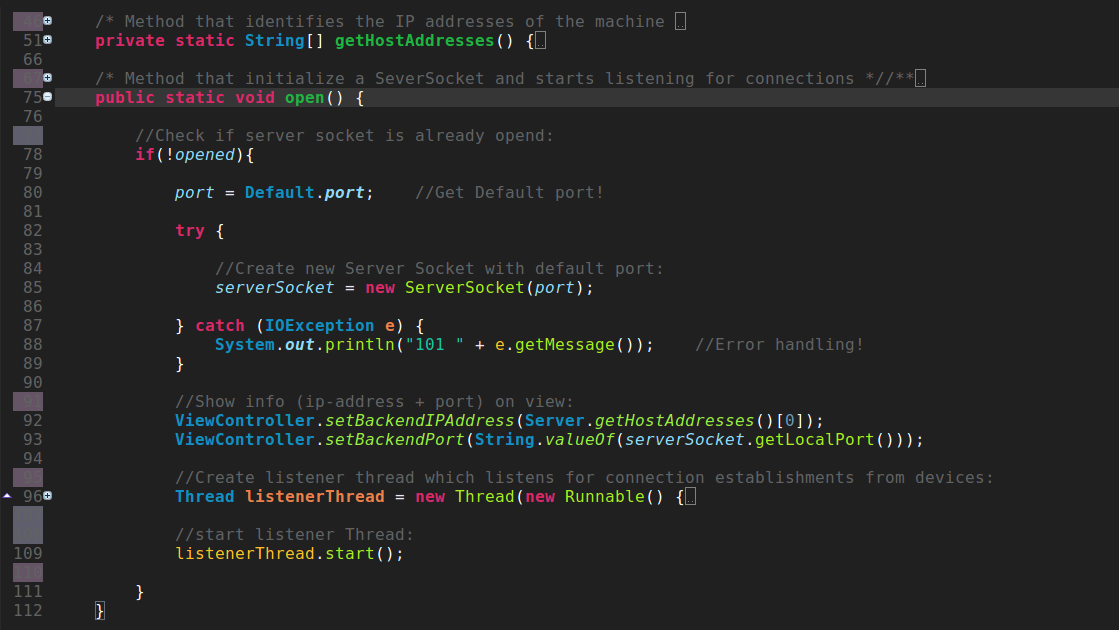
\includegraphics[width=1.0\textwidth]{images/implementation/SeverOpenMethod.png}
	\caption[\code{open()}-Methode der Sever-Klasse im Backend]{\code{open()}-Methode der Sever-Klasse im Backend}
\end{figure}
Nach der Initialisierung des Server-Socket wird ein Thread gestartet (listenerThread), welcher zyklisch die Methode \code{listen()}
aufruft. Die Aufgabe dieses Threads ist es kontinuierlich auf Verbindungsaufbauwünsche durch Roboter oder Apps zur warten und bei
deren eintreffen diese zu verarbeiten. \\
Die Abbildung X zeigt die Methode \code{listen()} in der ankommende Verbindungsaufbauwünsche verarbeitet werden.
\begin{figure}[ht]
	\centering
	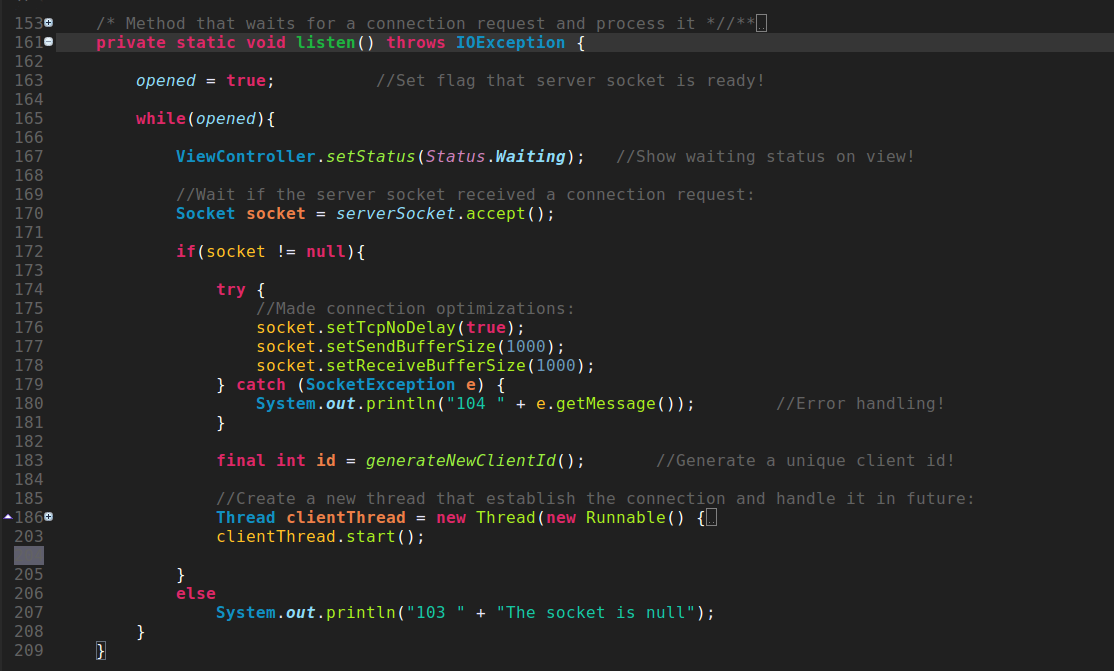
\includegraphics[width=1.0\textwidth]{images/implementation/SeverListenMethod.png}
	\caption[\code{listen()}-Methode der Sever-Klasse im Backend]{\code{listen()}-Methode der Sever-Klasse im Backend}
\end{figure}
Trifft ein Verbindungsaufbauwunsch ein wird für diesen, vom Server-Socket ein neues Socket Objekt zurück geliefert welches 
ab sofort eine unabhängige Verbindung zum anfangenden Device repräsentiert und ein Senden von Nachrichten in beide Richtungen 
ermöglicht.\\
Anschließend werden auf diesem Socket-Objekt noch ein paar Optimierungen durchgeführt um die Latenz der Kommunikation mit dem
Device möglichst gering zu halten. Dazu wird zum einen der Nagle-Algorithmus deaktiviert, siehe Abschnitt X sowie entsprechende
Puffergrößen festgelegt. \\
Danach wird ein Thread erzeugt der ab sofort die Kommunikation dieser Verbindung verwaltet. Dazu wird durch diesen ein neues Client-Objekt 
erzeugt, welches das zugehörige Socket-Objekt aufnimmt. Mit der Erzeugung dieses Client-Objekts, der Übergabe des Socket-Objekts und
der Zuordnung des Threads zur Verbindungsverarbeitung ist die Verbindung zu einem Device vollständig initialisiert und die Kommunikation 
zwischen Device und Backend kann beginnen. 
Ab sofort wird das entsprechende Device (App oder Robot) durch das Client-Objekt repräsentiert und kann durch dieses angesprochen werden. 
Innerhalb der Server Klasse werden sämtliche Clients (Instanzen der Klasse Client) in einer Listen-Datenstruktur (ArrayList) gespeichert 
und sind durch eine eindeutige ID identifizierbar.
\subsubsection{Client}
Neben der Server Klasse ist die Client Klasse eine zentrale Komponente der Kommunikation und ermöglicht das Senden von Daten an ein Device 
sowie Empfangen von Daten eines Devices.
Während die Server-Klasse auf Verbindungsaufbauwünsche der Geräte die sich am Backend anmelden wollen warten, und diese entgegen nimmt, 
repräsentieren die einzelnen Instanzen der Client Klasse eine Device und verwaltet die TCP-Verbindung zu diesem Device nach der Initialisierung
der Verbindung. \\
Dazu Verfügt das die Client Klasse über verschiedenen Attribute zur Kommunikation sowie zur Identifikation des durch die Instanz repräsentierten
Devices. Zur Kommunikation dienen folgende Attribute:
\begin{enumerate}
	%   ###############################################################################################################################
	\item{\code{private Socket socket}} -- Repräsentiert den TCP-Endpunkt zur Kommunikation mit dem Device.
	%   ###############################################################################################################################
	\item{\code{private BufferedReader bufferedReader}} -- Gepufferter Reader zu lesen von eintreffenden Datenpaketen.
	%   ###############################################################################################################################
	\item{\code{private OutputStream outputStream}} -- Stream zum versenden von Daten an das Device
	%   ###############################################################################################################################
	\item{\code{private Interpreter interpreter}} -- Instanz der Klasse Interpreter zum Parsen und Verarbeiten eintreffender Datenpakete
	%   ###############################################################################################################################
\end{enumerate}
Zur Identifikation des durch die jeweilige Client Instanz repräsentierten Devices nutzt das Programm folgende Attribute der Klasse:
\begin{enumerate}
	%   ###############################################################################################################################
	\item{\code{private ClientIdentification identification}} -- Identifikations-Objekt welches den Client eindeutig identifiziert.
	%   ###############################################################################################################################
	\item{\code{private Device device}} -- Referenz auf das ein konkretes Device-Objekt (Objekt der Klasse App oder Robot) welches die 
	Daten des Devices enthält mit dem durch den Client kommuniziert werden kann.
	%   ###############################################################################################################################
	\item{\code{private Szenario szenario}} -- Repräsentiert das Szenario, welchem das durch den Client dargestellte Device zugeordnet ist. 
	%   ###############################################################################################################################
\end{enumerate}
Die eigentliche Verarbeitung von Datenpaketen erfolgt in einem eigenen Thread der beim Verbindungsaufbau durch die Server-Klasse erzeugt wird und nach
Erzeugung des Client-Objekts sich um die Verarbeitung der vom Device gesendeten Datenpakete kümmert. Dazu prüft dieser zyklisch ob
Datenpakete am Backend eingetroffen sind, indem es das entsprechende BufferedReader-Objekt des Client-Objekts abfragt. Ist dies der Fall
wird das Datenpaket aus dem BufferedReader ausgelesen und als String-Objekt dem Interpreter-Objekt der Client-Instanz übergeben welches
das Datenpaket in ein JSON-Objekt konvertiert und weiter verarbeitet.
\subsubsection{Interpreter}
Die Interpreter Klasse ist zuständig für die Interpretation der am Backend eintreffenden Datenpakete der verschiedenen Devices. Dazu enthält
jedes Client-Objekt eine eigene Instanz der Klasse Interpreter, so dass eine parallele Verarbeitung ohne Beeinflussungen oder Wartezeiten 
möglich ist. \\
Die Interpretation der Datenpakete besteht aus zwei grundlegenden Schritte:
\begin{enumerate}
	%   ###############################################################################################################################
	\item{Parsen des als String vorliegenden Datenpakets in ein JSON-Objekt}
	%   ###############################################################################################################################
	\item{Weiterverarbeitung des JSON-Objekts anhand des vorliegenden Kommandotyps}
	%   ###############################################################################################################################
\end{enumerate}
Den ersten Schritt realisiert die Methode \code{public void parse(String pCommand)}. Zur Umwandlung des vorliegenden Strings verwendet
die Methode dazu eine Funktionalität der Bibliothek >>org.json<<. Anschließend wird das geparste JSON-Object abhängige von seinem
Kommandotyp durch eine entsprechende Methode weiterverarbeitet. \\
Die Abbildung X zeigt den Quellcode des Parse-Vorgangs in der Methode Vorgangs \code{public void parse(String pCommand)}.
\begin{figure}[ht]
	\centering
	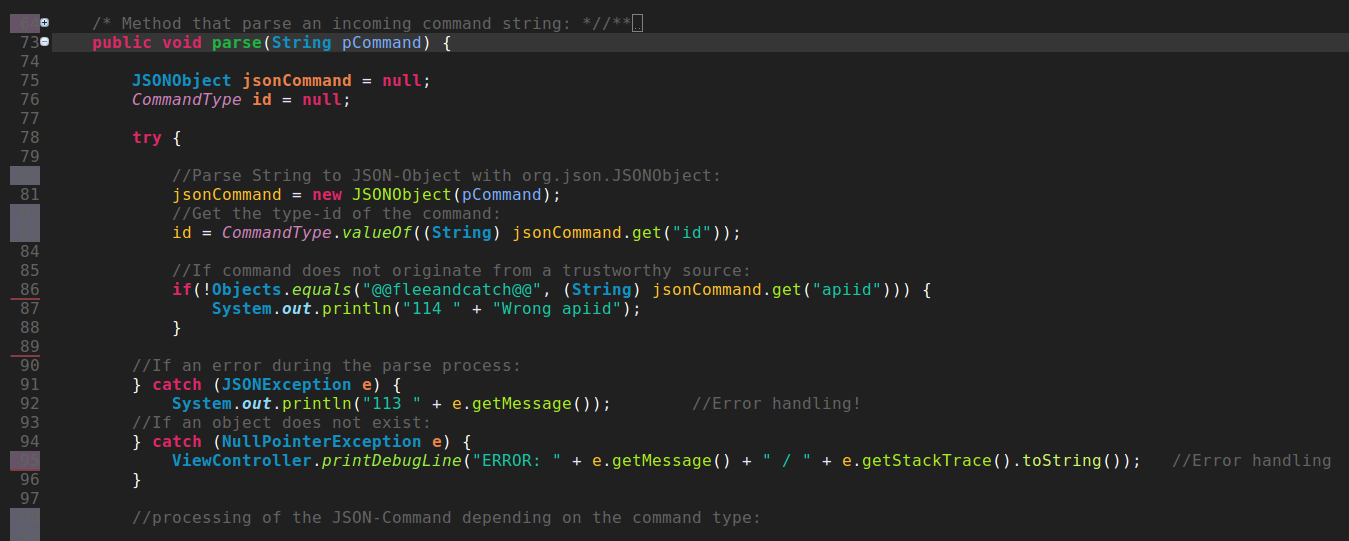
\includegraphics[width=1.0\textwidth]{images/implementation/InterpreterParseMethod.png}
	\caption[Ausschnitt der \code{parse()}-Methode der Interpreter-Klasse im Backend]{Ausschnitt der \code{parse()}-Methode der Interpreter-Klasse im Backend}
	\label{fig:ev3system}
\end{figure}
\newline
Die folgende Auflistung zeigt die Methoden der Interpreter Klasse:
\begin{itemize}
	%   ###############################################################################################################################
	\item{\code{public void parse(String pCommand)}} -- Diese Methode führt den eigentlichen Parse-Vorgang durch um das als String
	vorliegende Datenpaket (pCommand) in ein JSON-Objekt zu konvertieren.
	%   ###############################################################################################################################
	\item{\code{private void connection(JSONObject pCommand)}} -- Verarbeitet ein als JSON-Objekt vorliegendes Datenpaket vom Typ 
	Kommandotyp Connection.
	%   ###############################################################################################################################
	\item{\code{private void synchronization(JSONObject pCommand)}} -- Verarbeitet ein als JSON-Objekt vorliegendes Datenpaket vom 
	Typ Kommandotyp Synchronization.
	%   ###############################################################################################################################
	\item{\code{private void szenario(JSONObject pCommand)}} -- Verarbeitet ein als JSON-Objekt vorliegendes Datenpaket vom Typ 
	Kommandotyp Szenario. Dazu existieren folgenden folgende Methoden die die Daten abhängig vom vorliegenden Szenario verarbeiten:
	\begin{itemize}
			%   ###############################################################################################################################
			\item{\code{private void szenarioControl(SzenarioCommand pCommand)}}
			%   ###############################################################################################################################
			\item{\code{private void szenarioSynchron(SzenarioCommand pCommand)}}
			%   ###############################################################################################################################
			\item{\code{private void szenarioFollow(SzenarioCommand pCommand)}}
			%   ###############################################################################################################################
	\end{itemize}
	%   ###############################################################################################################################
	\item{\code{private void exception(JSONObject pCommand)}} -- Verarbeitet ein als JSON-Objekt vorliegendes Datenpaket vom Typ 
	Kommandotyp Exception.
	%   ###############################################################################################################################
\end{itemize}
Aus der Auflistung ist gut ersichtlich das es für jeden Kommandotyp eine eigene Methode zu dessen Verarbeitung implementiert wurde.
%\paragraph{Die \code{private void connection(JSONObject pCommand)} Mathode} verarbeitet Datenpakete welche die Kommunikation 
%mit den Devices betreffen. 
%Da diese in ähnlicher Art und Weise die Datenverarbeitung vornehmen wird im folgenden exemplarisch auf eine dieser Methode 
%eingegangen um dieses Prinzip zu verdeutlichen. \\
\subsubsection{Device \& Szenario Controller}
Neben den für die Kommunikation wichtigen Komponenten spielen bei der Realisierung des Backends auch die Controller-Klassen eine 
zentrale Rolle, da diese wichtige Verwaltungsfunktionen bereit stellen. Sie sind für die Verwaltung der verschiedenen Devices 
und Szenarien zuständig. \\
Dazu existieren die folgenden Controller-Klassen:
\begin{itemize}
	%   ###############################################################################################################################
	\item{AppController} -- Der AppContoller verwaltet alle am Backend angemeldeten Apps.
	%   ###############################################################################################################################
	\item{RobotContoller} -- Der RoboterContoller verwaltet alle am Backend angemeldeten Roboter.
	%   ###############################################################################################################################
	\item{ScenarioController} -- Der AppContoller verwaltet sämtliche aktiven Szenarien.
	%   ###############################################################################################################################
\end{itemize}
Die beiden Klassen AppController und RoboterController bestehen im wesentlichen aus einer Listen-Datenstruktur (ArrayList), in 
welcher sämtliche Apps bzw. Roboter die am Backend angemeldet sind gespeichert werden. In dieser Datenstruktur werden die Devices 
durch Objekte entsprechender Klassen (App-Klasse, Roboter-Klasse) repräsentiert. \\
Die Controller-Klassen verfügen über Datenstrukturoperationen zum Einfügen, Entfernen, Suchen oder zum Aktualisieren von Elementen
so das durch entsprechende Methoden eine einfacher Zugriff auf die Devices sowie deren Manipulation möglich ist. \\
Da alle drei Controller-Klassen mit statischen Datenstrukturen und Methoden arbeiten werden die angemeldeten Devices zentral 
gespeichert und Verwaltet was einen einfachen und schnellen Zugriff auf diese ermöglicht und Redundanzen und Inkonsistenzen vermeidet.
Durch die Verwendete Listen-Datenstruktur ist ein einfaches Suchen, Einfügen sowie Löschen möglich. Zudem kann leicht über die 
einzelnen Devices iteriert werden was hilfreich ist wenn die selben Daten an mehrere Devices gesendet werden müssen.
\\
Die SzenarioController Klasse verfügt über die gleiche Listen-Datenstruktur zur Speicherung von Szenarien, jedoch bietet sie neben
den Einfachen Operatoren noch weitere Komplexere Funktionalitäten zum Abfragen ob bestimmte Devices am Szenario teilnehmen etc. 
\subsubsection{Die GUI}
Neben den rein Funktionalen Komponenten des Backends verfügt dieses auch über eine grafische Benutzeroberfläche die Informationen zu
den angemeldeten Geräten und den existierenden Szenarien zur Verfügung stellt. Diese Benutzeroberfläche ist so realisiert das diese 
komplett losgelöst von den der eigentlichen Funktionalität des Backend ist. Sie setzt lediglich auf dem eigentlichen Programm auf und
ist zu dessen Ausführung nicht notwendig. Dadurch ist es möglich das Programm komplett ohne grafische Benutzeroberfläche zu starten so
das es im Hintergrund laufen kann und lediglich als Verwaltungs- und Kommunikationsservice dient. Ob die grafische Benutzeroberfläche  
aktiviert ist oder nicht wird beim Programmstart durch entsprechenden Parametern festgelegt. \\
Der Nutzen der GUI bestand für uns hauptsächlich im Monitoring und bei der Identifikation sowie dem Aufspüren von Fehlern während der 
Entwicklung. \\
Realisiert ist die grafische Benutzeroberfläche mit dem JavaFX-Framework welches Bestandteil der Java-Bibliothek ist uns somit wie 
Java ebenfalls plattformunabhängig lauffähig ist. Zu ihrer Ansteuerung dient eine spezielle Klasse namens
>>ViewController<< welche lediglich Informationen des eigentliche Programms entgegen nimmt und an die eigentliche Benutzeroberfläche 
(View) weiterreicht sofern diese aktiviert wurde. Umgekehrt werden jedoch keine Benutzereingaben von der GUI an das Programm 
weitergereicht, sondern dienen lediglich zur Manipulation der Anzeige so das dieses komplett unabhängig ist. Lediglich das Beenden 
das kompletten Programms ist über die grafische Benutzeroberfläche möglich.
Abbildung X.X zeigt einen Screenshot der grafischen Benutzeroberfläche des Backends.
\begin{figure}[ht]
	\centering
	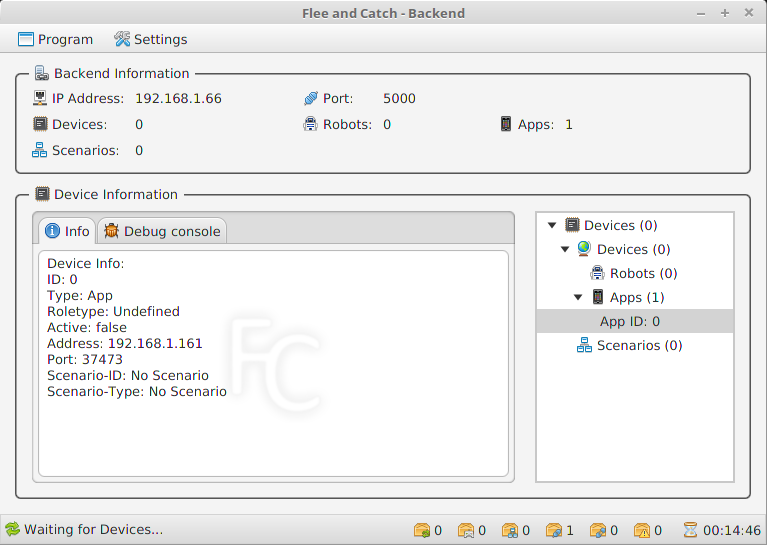
\includegraphics[width=1.0\textwidth]{images/implementation/BackendGUI.png}
	\caption[Grafische Benutzeroberfläche des Backends]{Grafische Benutzeroberfläche des Backends}
\end{figure}
\newline
Da die grafische Benutzeroberfläche jedoch nicht zur eigentlichen Funktionalität des Backends beiträgt soll an dieser Stelle nicht 
weiter eingegangen werden.
\newpage
\subsection{Roboter}
Die Implementierung des Roboters stellt das Kernstück bei der Realisierung dieses Projekts dar. Durch die Programmierung der
EV3-Roboter wird deren letztendliches Verhalten d.h. die Datenerfassung sowie ihre Bewegung bestimmt. Da die durch die Datenerfassung 
die berechneten Positionsdaten die Grundlage zur Berechnung der Verfolgungssteuerung bilden muss diese möglichst exakt erfolgen.
Im Gegenzug dazu bestimmt Programmierung der Steuerung die resultierenden Bewegung der Roboter und ist somit maßgeblich für die 
Abbildung der veranschlagten Szenarien die ein Schwarmverhalten nachbilden sollen. \\
Die nachfolgenden Abschnitte beschreiben den Aufbau des Roboterprogramms sowie die notwendigen Komponenten wie Klassen und 
Threads, die zur Kommunikation, Datenerfassung als auch Steuerung notwendig sind und erläutert die dahinter stehenden Konzepte 
und Prinzipien.
\subsubsection{Aufbau \& Klassenstruktur}
%\color{finishing}             % Farbe die angibt welchen Status der folgende Abschnitt hat!
% Eigentlicher Text:
Zur Strukturierung und einer sauberen Trennung der einzelnen Klassen und ihren Sichtbarkeiten, sind diese in verschiedenen 
Paketen (Java-Packages) organisiert. Diese Klassenstruktur ist hierarchisch aufgebaut, orientiert sich an den grundlegenden 
Bestandteilen des Programms (Kommunikation, Roboterkontrolle etc.) und granuliert in einzelnen Unterpakete anhand der Objekten 
welche die jeweiligen Klassen darstellen bzw. welche Funktionen diese bieten. \\
Bei der Umsetzung wurden die Klassen in den folgenden vier großen Paketbereiche strukturiert.
\begin{itemize}
	%   ###############################################################################################################################
	\item{Kommunikation (\code{flee\_and\_catch.robot.communication})} -- Enthält sämtliche Klassen die für die Kommunikation mit dem
	Backend notwendig sind dazu zählen die Eigentlichen Kommunikator (Sockets), die verschieden Kommandos sowie serialisierbare 
	Datenobjekte.
	%   ###############################################################################################################################
	\item{Roboter (\code{flee\_and\_catch.robot.robot})} -- Hier befinden sich alle Klassen die direkten Zugriff bzw. Einfluss auf den 
	physischen Roboter haben. Dies sind hauptsächlich Sensoren, das Roboter-Interface, Klassen die einen konkreten Roboter darstellen, 
	sowie die zentrale Steuerklasse >>RoboterController<<.
	%   ###############################################################################################################################
	\item{View (\code{flee\_and\_catch.robot.view})} -- Enthält Klassen die der Anzeige d.h Ansteuerung des LCD-Displays des
	Roboters dienen. Zwar ist das LCD-Display auch Bestandteil des Roboters, es wurde sich aber für eine Trennung dieser beiden 
	Bereiche entschieden da diese möglichst unabhängig voneinander bleiben sollten.
	%   ###############################################################################################################################
	\item{Konfiguration (\code{flee\_and\_catch.robot.configuration})} -- Zentrales Paket welches Klassen zur Konfiguration 
	der verschiedenen Programmteile enthält.
	%   ###############################################################################################################################
\end{itemize}
Innerhalb dieser Hauptpakete existieren zahlreiche weitere Unterpakete welche die Klassen weiter strukturieren. Die saubere Einordnung
und Trennung der Programmklassen ermöglicht es in Verbindung mit der Festlegung entsprechender Sichtbarkeiten, die Klassen gegeneinander 
abzuschotten. So wird erreicht, dass die Programmteile lediglich über die vorgesehenen Schnittstellen miteinander interagieren und die
einzelnen Klassen nur diejenigen sehen und ansprechen können die sie tatsächlich benötigen. Zudem hilft es dem Programmierer bei der 
Orientierung und dem Programmverständnis.
%\medskip
%\newline
%In den nächsten Abschnitten werden die wichtigsten Klassen und Interfaces des Programms näher beschrieben und ihre Rolle bei der 
%Realisierung des durch die Roboter abgebildeten Schwarmverhaltens erläutern.
\subsubsection{Threads}
Für die Umsetzung der Szenarien ist es erforderlich das der Roboter verschiedene Dinge parallel erledigt. Zum einen muss die 
ständige und zeitnahen Kommunikation mit dem Backend aufrecht erhalten werden, um zum einen Steuerdaten sowie die Positionsdaten
der anderen Roboter für die Bewegungsberechnung zu empfangen. Andererseits müssen über diese Verbindung die eigenen Daten übermittelt
an das Backend übermittelt werden. Darüber hinaus muss die eigentliche Steuerung des Roboters erfolgen. \\
Zur Realisierung all dieser Aufgaben sind innerhalb des Roboters die folgenden X Threads implementiert:
\begin{itemize}
	%   ###############################################################################################################################
	\item{Hauptthread (main thread)}
	%   ###############################################################################################################################
	\item{Thread zur Überprüfung der Kommunikationsinitiierung (connectionThread)}
	%   ###############################################################################################################################
	\item{Daten-Empfangs-Thread (listenThread)}
	%   ###############################################################################################################################
	\item{Steuerungsthread (steeringThread)}
	%   ###############################################################################################################################
	\item{Daten-Sende-Thread (synchronizeThread)}
	%   ###############################################################################################################################
\end{itemize}
In den folgenden Abschnitten werden die einzelnen Threads sowie ihre Aufgaben dargestellt:
\paragraph{Hauptthread}
Der Hauptthread ist der Thread welcher beim Programmstart (Aufruf der Funktion public static void main(String[] args)) automatisch 
erzeugt wird und der immer vorhanden ist. Durch diesen Thread werden in der Initialisierungsphase die Verbindung zum Backend initiiert 
sowie alle weiteren Threads für die Kommunikation, Steuerung und Datenerfassung erzeugt. 
\paragraph{Thread zur Überprüfung der Kommunikationsinitiierung}
Dieser Thread dient der Überprüfung einer korrekten Initiierung der Kommunikation mit dem Backend. Dazu wird dieser während der 
Initiierungsphase erzeugt und prüft im 100 Millisekunde Takt zyklisch ob eine Verbindung zum Backend aufgebaut werden konnte. Wurde
innerhalb von 3 Sekunden keine Verbindung aufgebaut wird durch den Thread ein Fehler gemeldet.
\paragraph{Daten-Empfangs-Thread}
Dieser Thread lauscht auf der TCP-Verbindung ob Pakete vom Backend eintreffen ließt diese als String aus und übergibt diesen der 
Interpreter-Klasse um das Datenpaket in ein JSON-Objekt zu konvertieren und weiter zu verarbeiten.
\paragraph{Steuerungsthread}
Der Steuerungsthread hat wie der Name schon sagt die Aufgabe den Roboter zu steuern das heiß seine Geschwindigkeit und Bewegungsrichtung 
umzusetzen. Implementiert ist der Steuerungsthread in der RobotController Klasse die als Schnittstelle zwischen der Kommunikation und den
Roboterfunktionalitäten fungiert. \\
Die konkrete Umsetzung der Steuerung die durch diesen Thread erfolgt wird im Abschnitt X.X beschrieben.
\paragraph{Daten-Sende-Thread}
Neben dem Empfangen von Daten und der Umsetzung der Steuerung muss der Roboter auch seine eigen Daten wie Position, Orientierung und 
Geschwindigkeit kontinuierlich erfassen und an das Backend übermitteln so das diese Informationen den anderen Robotern zur Verfügung
gestellt werden können. Da dieser Thread dazu auf Funktionalitäten des Roboters zugreift ist auch dieser innerhalb der RoboterController
Klasse implementiert.
\\
Die Realisierung der Datenerfassung wird im Abschnitt X.X beschrieben.
\medskip
\newline
Die Abbildung X.X zeigt das Zusammenspiel der einzelnen Threads bzw. den Ablauf ihrer Erzeugung und Terminierung:
\subsubsection{Klassen}
Neben den verschiedenen Threads enthält das Roboterprogramm zahlreiche Klassen durch welche die vielfältigen Funktionen abgebildet 
werden die, der Roboter zur Realisierung der verschiedenen Szenarien mitbringen muss. 
\paragraph{Das Roboter Interface}
dient als Implementierungsvorlage für Klassen die einen Roboter in seiner jeweiligen physischen Gestalt d.h. mit
der jeweiligen Antriebsform, seinen verbauten Sensoren etc darstellen. Innerhalb dieses Interfaces sind sämtliche Funktionalitäten 
und Methoden definiert, die ein konkreter Roboter bzw. die entsprechende Klasse, die diesen repräsentiert implementieren muss um durch 
das Programm gesteuert und in die entsprechenden Szenarien integriert werden zu können. \\
Innerhalb dieses Interface werden dazu verschiedene Methoden zur Steuerung sowie Abfrage von Roboterparametern definiert. Die durch 
diese Methoden dargestellten Funktionalitäten sind von so grundlegender Natur das diese durch jeden Roboter realisiert bzw. umgesetzt 
werden können, wenn auch abhängig von seiner Bauart auf andere Weise. \\
Folgende Auflistung gibt einen Überblick über die wichtigsten diese Methoden und erläutert kurz die durch sie zur realisierende Funktion.
\begin{itemize}
	%   ###############################################################################################################################
	\item{\code{void forward()}} -- Soll den Roboter geradeaus vorwärts fahren lassen.
	%   ###############################################################################################################################
	\item{\code{void backward()}} -- Soll den Roboter geradeaus rückwärts fahren lassen.
	%   ###############################################################################################################################
	\item{\code{void backward()}} -- Soll den Roboter sich nach rechts oder linkes bewegen lassen abhängig von der übergebenen Richtung
	(Direction-Objekt).
	%   ###############################################################################################################################
	\item{\code{void stop()}} -- Soll den Roboter anhalten.
	%   ###############################################################################################################################
	\item{\code{void increaseSpeed()}} -- Soll die Geschwindigkeit des Roboters erhöhen (Iterativ bei jedem Aufruf).
	%   ###############################################################################################################################
	\item{\code{void increaseSpeed()}} -- Soll die Geschwindigkeit des Roboters verringern (Iterativ bei jedem Aufruf).
	%   ###############################################################################################################################
	\item{\code{boolean isMoving()}} -- Soll true zurückgeben wenn sich der Roboter bewegt.
	%   ###############################################################################################################################
	\item{\code{Position getPosition()}} -- Soll die aktuelle Position und Orientierung des Roboters in einem speziellen 
	Position-Objekt zurückgeben.
	%   ###############################################################################################################################
	\item{\code{float getRealSpeed()}} -- Soll tatsächliche (nicht eingestellte) Geschwindigkeit des Roboters zurückgeben.
	%   ###############################################################################################################################
	\item{\code{Robot getJSONRobot()}} -- Soll alle wichtigen Roboterdaten einem speziellen Roboter-Objekt zurückgeben welches 
	serialisierbar ist und damit via JSON-Objekt an des Backend übertragen werden kann.
	%   ###############################################################################################################################
\end{itemize}
Durch die Vorgaben und Verwendung dieser grundlegenden und universellen Funktionalitäten für die Programm-, Szenarien- und Steuerlogik 
ist es mögliche eine generische und flexible Implementierung zu schaffen. Da ein Roboter immer als Objekt dieses Interfaces betrachtet 
und angesprochen wird ist das restliche Programm vollkommen unabhängig von der konkreten Ausprägung des jeweilige Roboter und kennt 
diese nicht mal. Es beschränkt sich bei der Interaktion mit dem Roboter auf die in diesem Interface definierten Methoden. \\
Der Vorteil dieser Implementierung liegt darin, dass durch dieses generische Programmierung lediglich eine neuen Klasse die dieses 
Interface implementiert notwendig ist um einen neue Art von Roboter zu Realisierung und in das Projekt mit sämtlichen Szenarien zu 
integrieren. Dadurch ist das Programm leicht erweiterbar und es steigert seine Wiederverwendbarkeit. \\
Wie diese konkrete Implementierung der durch diese Methoden definierten Funktionen zu realisieren ist hängt natürlich vom jeweilige
Roboter und seinem Aufbau ab und muss durch den Programmiere entsprechend umgesetzt werden.
\pagebreak
\begin{wrapfigure}{r}{0.30\textwidth}
	\vspace{+0.0cm}
	\begin{center}
		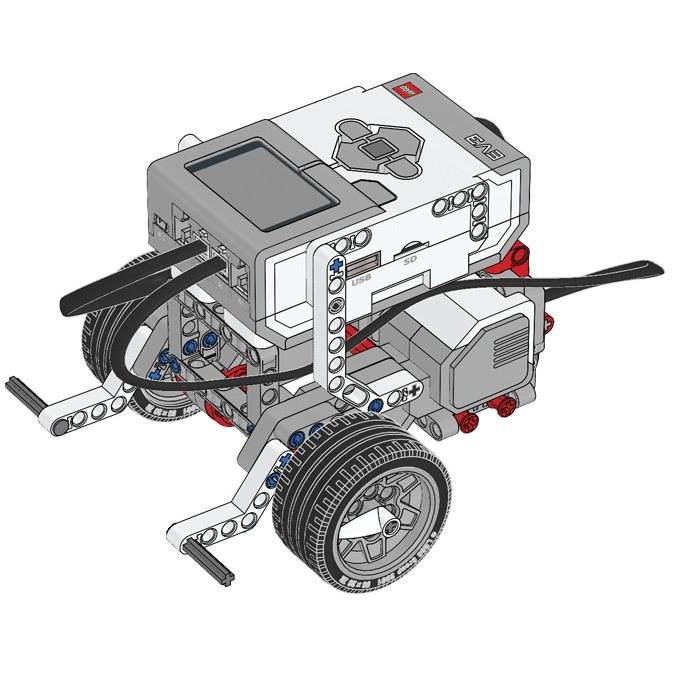
\includegraphics[width=0.25\textwidth]{images/implementation/threewheeldrive.png}
	\end{center}
	\caption{Dreirad-Antrieb}
	\label{fig:einachsenlenkung}
\end{wrapfigure}
\paragraph{Die ThreeWheelDrive Klasse}
\color{process}             % Farbe die angibt welchen Status der folgende Abschnitt hat!
% Eigentlicher Text:
repräsentiert im Roboterprogramm den \glqq{}Standard\grqq{}-Roboter des Projekts. Sie beschreibt somit einen konkreten 
Robotertyp in seinem Aufbau. Sie bildet den in Abbildung X.X zu sehenden Roboter (Auf der Abbildung fehlt der Ultraschall- und Gyrosensor) 
mit seine relevanten Komponenten wie Sensoren, 
Motoren sowie geometrischen und physischen Parametern ab. Die Klasse implementiert das Roboter-Interface mit den dort definierten 
Methoden und setzt die jeweilige Funktionalität für diesen Robotertyp um.\\
Neben diesen Schnittstellen Methoden verfügt diese Klasse über zahlreiche Attribute wie Motor- und Sensor-Objekte aus der 
EV3-Bibliothek sowie spezielle Hilfsfunktionen die es ermöglichen den Roboter und seine Komponenten so anzusteuern das er die im 
Roboter-Interface definierten Aktionen ausführen kann. Diese Attribute und Hilfsfunktionen sind jedoch nach Außen hin nicht
sichtbar und verbergen so die Komplexität und Individualität des Roboters vor dem restlichen Programm insbesondere vor dem 
RoboterController. \\
Die folgende Abbildung gibt eine Einblick über die verschiedenen EV3-Bibliothekskompo\-nenten die bei der Realisierung des 
ThreeWheelDrive-Roboters Anwendung finden:
\begin{itemize}
	%   ###############################################################################################################################
	\item{\code{private EV3MediumRegulatedMotor motorRight, motorLeft;}} -- Das EV3\-Medium\-RegulatedMotor-Objekt der EV3-Java-Bibliothek
	repräsentiert eine mittleren Motor des EV3-Sets mit integrierten Rotationssensor. Zur Realisierung des ThreeWheel\-Drive-Roboters
	sind für den Differentialantrieb zwei dieser Motor-Objekte notwendig.
	%   ###############################################################################################################################
	\item{\code{private Ultrasonic ultrasonic}} -- Das Ultrasonic-Objekt repräsentiert den Ultraschallsensor des Roboters mit dem der 
	Abstand zu einem Hindernis ermittelt werden kann und der zur Notabschaltung vor einer Kollision dient.
	%   ###############################################################################################################################
	\item{\code{private Gyro gyro}} -- Durch die Instanz der Klasse Gyro wird der Gyrosensor des Roboters abgebildet welcher in unserem
	Projekt zur Verifizierung der durch Odometrie ermittelten Position und Orientierung des Roboters vorgesehen war.
	%   ###############################################################################################################################
\end{itemize}
Neben den Sensor und Motor-Elementen sind auch physische Parameter des Roboters für die Datenerfassung und Steuerung notwendig wie
beispielsweise die folgenden Parameter:
\begin{itemize}
	%   ###############################################################################################################################
	\item{\code{public static final float DISTANCE\_DEGREE =   0.476389f;}} -- Dieser Parameter gibt an die Distanz in Millimetern 
	an die sich ein Rad bei der Drehung um 1 Grad vorwärts bewegt.  
	%   ###############################################################################################################################
	\item{\code{public static final float DIAMETER\_WHEELS = 120.000000f;}} -- Dieser Parameter gibt den Abstand der Beiden Räder 
	des Differentialantriebs in Millimetern an.
	%   ###############################################################################################################################
\end{itemize}
Über welche Methoden bzw. die durch diese repräsentierten Funktionen die jeweilige Komponenten verfügen und wie diese angesteuert 
werden, wird im Abschnitt X.X bei der Implementierung der Robotersteuerung erläutert.
\paragraph{Die RoboterController Klasse} übernimmt eine zentrale Rolle bei der Umsetzung der Roboter-Steuerung. Die Klasse stellt die 
Schnittstelle zum physischen Roboter dar. Sämtliche Steuerkommandos und Sensorabfragen werden über diese Klasse realisiert. Durch diese einheitliche 
Schnittstelle wird es möglich die Steuerung und ... unabhängig von dem konkreten vorhandenen Roboter (Dreirädriger, Vierrädriger etc)
zu realisieren. Dazu nutzt der RoboterController intern eine Instanz des "Roboter" Interfaces was eine Ansteuerung des Roboters 
\\
\subsubsection{Steuerung}
Eine der Hauptaufgaben des Roboterprogramms ist die Steuerung des Roboters. Dabei muss das Programm die folgende zwei 
grundlegenden Steuerungsarten unterscheiden und realisieren.
\begin{itemize}
	%   ###############################################################################################################################
	\item{Direkte Steuerung} -- Bei der direkten Steuerung erhält das Programm über das Backend von der App direkte Steuerbefehle wie
	Rechts, Links, Schneller, Langsamer welche das Programm dann in die entsprechende Bewegung des Roboters umsetzen muss.
	%   ###############################################################################################################################
	\item{Indirekte Steuerung} -- Bei der indirekten Steuerung bekommt das Programm keinen konkreten Steuerbefehle sondern muss basierend
	auf den Positionsdaten der anderen Roboter und dem vorherrschenden Szenario die notwendigen Steuerbefehle des Roboters berechnen.
	%   ###############################################################################################################################
\end{itemize}
Dabei erfolgt das Empfangen und Verarbeiten der jeweiligen Daten jeweils zyklisch in einem konfigurierbaren Zeitintervall. Beide Steuerungsarten
basieren auf dem grundlegenden Prinzip, dass die vom Backend gesendeten Daten (Steuerbefehle oder Positionsdaten) durch den 
Daten-Empfangs-Thread (listenThread) empfangen, verarbeitet und in entsprechenden Objekten der RoboterController-Klasse gespeichert werden. 
Dieser Vorgang erfolgt zyklisch und vollständig unabhängig von der eigentlichen Umsetzung der Steuerung durch den Steuerungsthread (steeringThread). \\
Der Steuerungsthread wiederum liest die gespeicherten Positions- bzw. Steuerdaten aus und führt auf deren Basis entsprechenden Roboterbefehle 
aus um die gewünschte Steuerung zu realisieren.
\begin{figure}[ht]
	\centering
	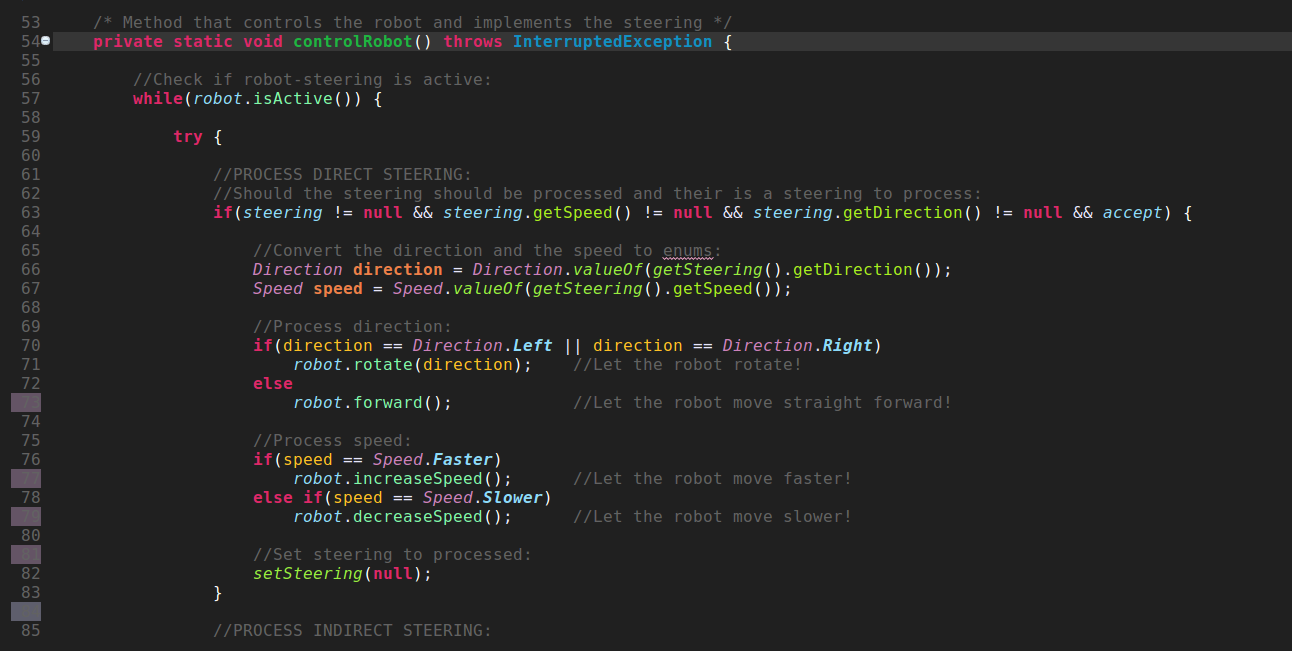
\includegraphics[width=1.0\textwidth]{images/implementation/controlRobotMethod1.png}
	\caption[\code{controlRobot()}-Methode der RobotController-Klasse im Robot]{\code{controlRobot()}-Methode der RobotController-Klasse im Robot}
\end{figure}
\newline
Die Abbildung X zeigt einen Ausschnitt der Methode \code{controlRobot()} innerhalb der RobotController-Klasse. Der in der Abbildung zu 
sehende Quellcode realisiert die direkte Steuerung des Roboters durch die beim Roboter eintreffenden Steuersignale der App. Die 
\code{controlRobot()}-Methode wird durch den Steuerungsthread zyklisch aufgerufen um eine permanente Steuerung ohne Zeitverzögerung
zu erreichen. \\
Innerhalb der Methode wird zuerst geprüft ob der Roboter überhaupt aktiv ist d.h. an einem Szenario teil nimmt und überhaupt gesteuert werden
muss. Anschließend wird geprüft ob ein Befehl zur direkten Steuerung vorliegt. Dafür müssen die folgenden Bedingungen erfüllt sein:
\begin{itemize}
	%   ###############################################################################################################################
	\item{Es muss ein gültiges Steuerungskommando vorliegen}
	%   ###############################################################################################################################
	\item{Das Akzeptieren eins Steuerungskomando}
	%   ###############################################################################################################################
\end{itemize}
Die indirekte Steuerung wird ebenfalls in der \code{controlRobot()}-Methode realisiert ist jedoch um einiges komplexer und erfordert eine
Vielzahl von Überprüfungen, Fallunterscheidungen und Berechnungen, weshalb an dieser Stelle auf den Quellcode verwiesen wird.
\subsubsection{Datenerfassung \& Synchronisation}
Zur Erfassung der Daten des Roboters wie einer Position, Orientierung etc. und deren anschließenden Übermittlung an das Backend, 
existiert wie bereit erwähnt ein separater Thread (synchronizeThread). Die eigentliche Erfassen und Senden der Daten erfolgt in der 
\code{synchronize()}-Methode innerhalb der RoboterController-Klassen welche der synchronizeThread nach seiner Erzeugung betritt.
Abbildung X zeigt den Quellcode der \code{synchronize()}-Methode.
\begin{figure}[ht]
	\centering
	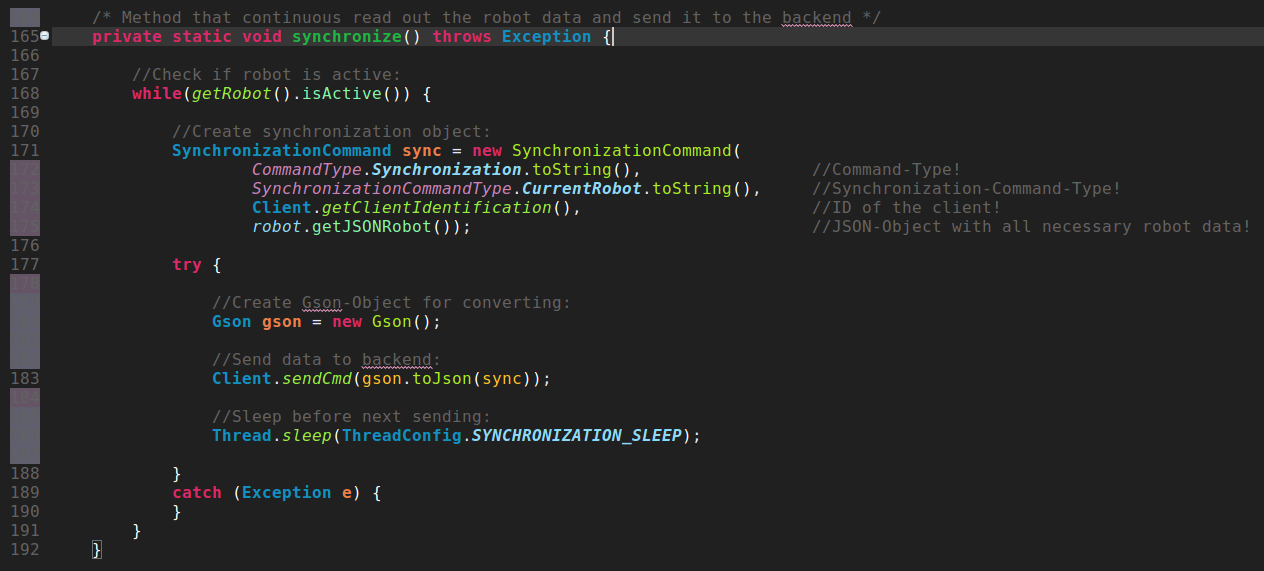
\includegraphics[width=1.0\textwidth]{images/implementation/synchronizeMethod.png}
	\caption[\code{synchronize()}-Methode der RobotController-Klasse im Robot]{\code{controlRobot()}-Methode der RobotController-Klasse im Robot}
\end{figure}
\newline
Is der Roboter aktiv d.h. nimmt an eine Szenario teil werden durch die Methode )zyklisch ein entsprechendes Synchronisations-Kommando erzeugt, welches
die aktuellen Roboterdaten enthält. Diese Daten werden vom Roboter durch den Aufruf der Methode {\code{getJSONRobot()} als spezielles serialisierbares 
Datenobjekt zurückgeliefert. Anschließend wird dieses Datenobjekt konvertiert und durch Aufruf der Funktion {\code{controlRobot()}. Nach abwarten einer 
konfigurierbare Zeit startet dieser Prozess von neuem. \\
Die Abbildung X zeigt die Implementierung der Funktion {\code{getJSONRobot()} in der Klasse ThreeWheelDrive welche das Datenobjekt mit den 
entsprechenden Roboterdaten erzeugt.
\begin{figure}[ht]
	\centering
	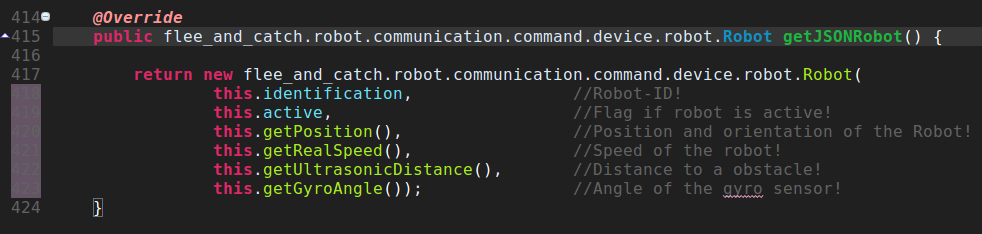
\includegraphics[width=1.0\textwidth]{images/implementation/getJSONRobotMethod.png}
	\caption[\code{synchronize()}-Methode der RobotController-Klasse im Robot]{\code{controlRobot()}-Methode der RobotController-Klasse im Robot}
\end{figure}
Zur eigentlichen Erfassung der Daten von den Robotersensoren und deren Aufbereitung nutzt der Roboter mehrere Methoden wie X und X.
Abbildung X zeugt exemplarich wie beim ThreeWheelDrive-Roboter die Position und Orientierung durch die Methode {\code{getPosition()} berechnet und
in einem Objekt der Klasse Position zurückgeliefert wird.
\begin{figure}[ht]
	\centering
	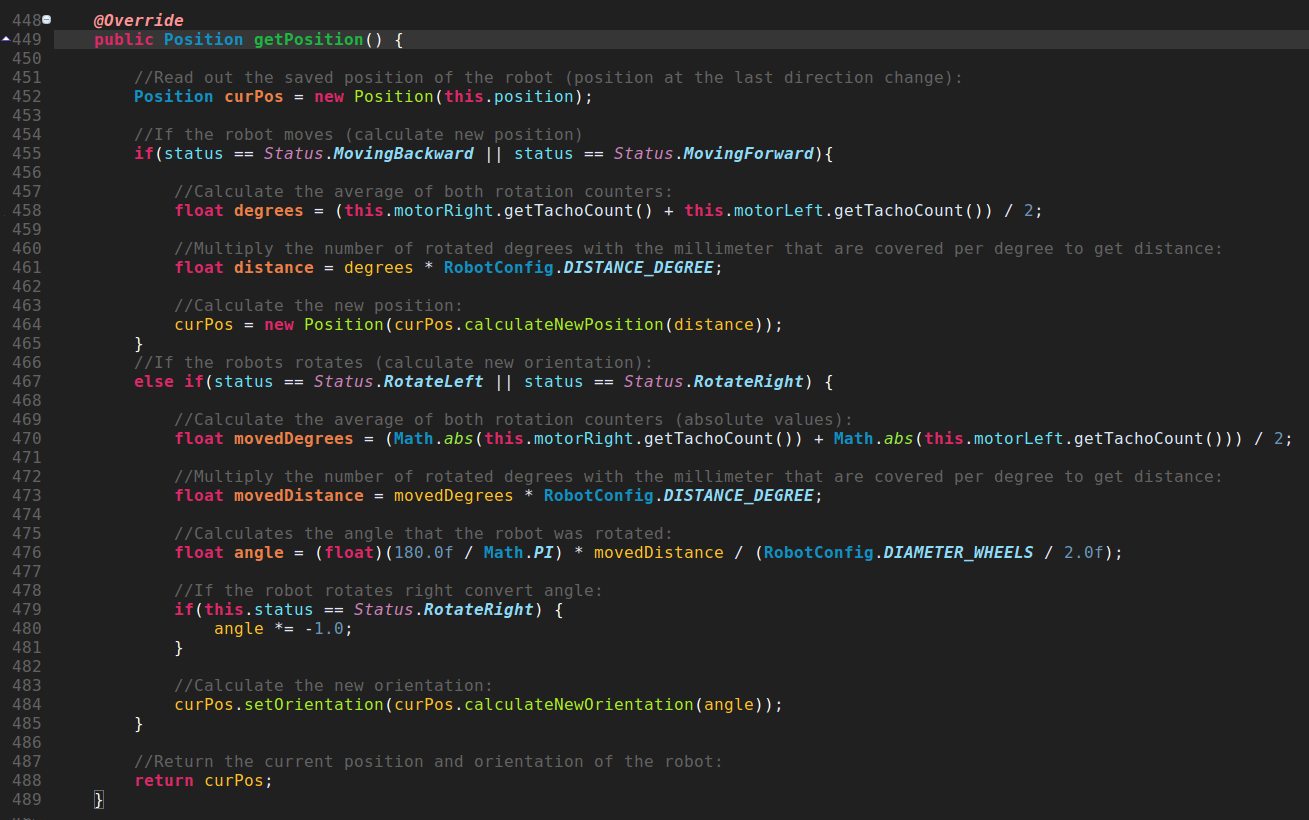
\includegraphics[width=1.0\textwidth]{images/implementation/getPositionMethod.png}
	\caption[\code{synchronize()}-Methode der RobotController-Klasse im Robot]{\code{controlRobot()}-Methode der RobotController-Klasse im Robot}
\end{figure}
\begin{figure}[ht]
	\centering
	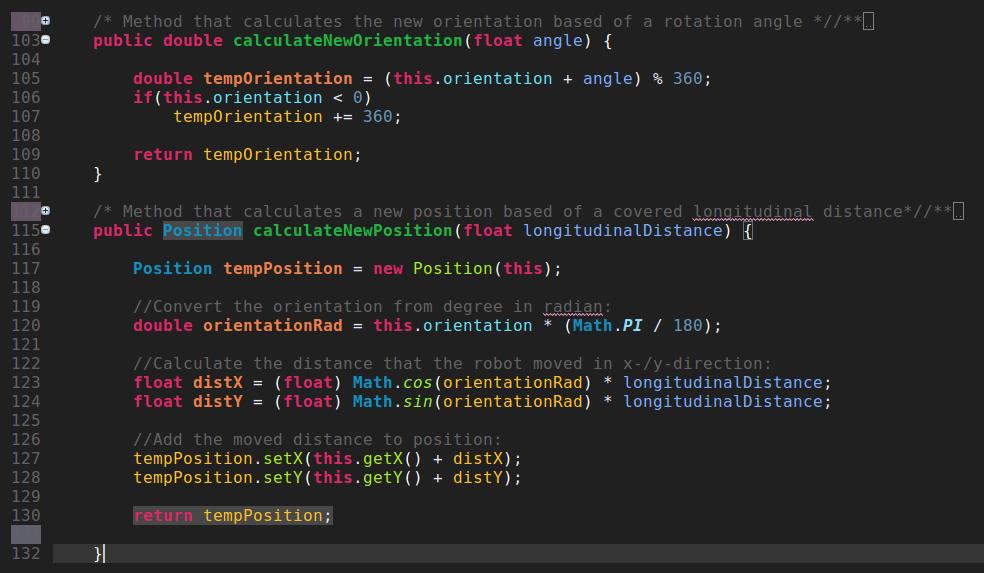
\includegraphics[width=1.0\textwidth]{images/implementation/positionMethods.png}
	\caption[\code{synchronize()}-Methode der RobotController-Klasse im Robot]{\code{controlRobot()}-Methode der RobotController-Klasse im Robot}
\end{figure}
asdsada